\documentclass[a4paper,12pt,twoside,openany]{report}
\usepackage{polski}
\usepackage[utf8]{inputenc}
\usepackage[pdftex]{graphicx}
\usepackage{tabularx}
\usepackage{array}
\usepackage[polish]{babel}
\usepackage{subfigure}
\usepackage{amsfonts}
\usepackage{verbatim}
\usepackage{indentfirst}
\usepackage{longtable}
\usepackage{supertabular}
\usepackage{xcolor}
\usepackage[pdftex]{hyperref}
\usepackage{geometry}

\newcommand{\ImgPath}{./img}
\newcommand{\TODO}{\textbf{TODO}}
\newcommand{\tech}{\texttt}

% na oprawe (1.0cm - 0.7cm)*2 = 0.6cm
% na oprawe (1.1cm - 0.7cm)*2 = 0.8cm
%  oddsidemargin lewy margines na nieparzystych stronach
% evensidemargin lewy margines na parzystych stronach
\def\oprawa{1.06cm}
\addtolength{\oddsidemargin}{\oprawa}
\addtolength{\evensidemargin}{-\oprawa}

% table span multirows
\usepackage{multirow}
\usepackage{enumitem}	% enumitem.pdf
\setlist{listparindent=\parindent, parsep=\parskip} % potrzebuje enumitem

%%%%%%%%%%%%%%% Dodatkowe Pakiety %%%%%%%%%%%%%%%%%
\usepackage{prmag}   % definiuje komendy opieku,nrindeksu, rodzaj pracy, ...


%%%%%%%%%%%%%%% Strona Tytułowa %%%%%%%%%%%%%%%%%
\title{Projektowanie architektury korporacyjnej z zastosowaniem języka SoaML}

\author{Mateusz Mróz}
\nrindeksu{221192}
\zdjecie{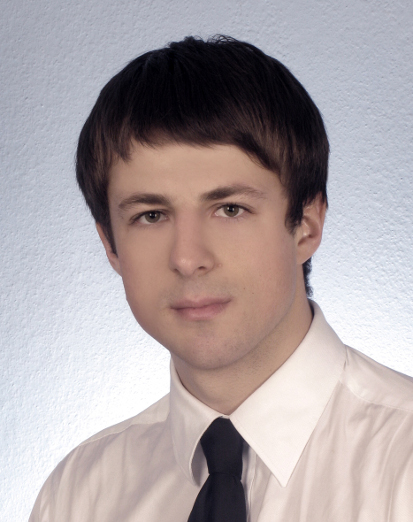
\includegraphics[width=4cm]{\ImgPath/zdjecie_legitymacja.jpg}}

\opiekun{dr inż. Włodzimierz Dąbrowski}
\terminwykonania{01.06.2015} % data złożenia - pokazana na stronie tytułowej
\datawydaniatematu{24 marca 2014}
\rokakademicki{2014/2015}

\begin{document}
\maketitle
\setcounter{secnumdepth}{3}
\setcounter{tocdepth}{3}
\tableofcontents
\chapter{Wstęp}
W ostatnich latach zarysowuje się coraz większa potrzeba wdrażania systemów informatycznych. Ta tendencja związana  jest przede wszystkim z usprawnianiem procesów biznesowych, ze wzrostem wydajności pracy, identyfikacją oraz minimalizacją błędów lub nieefektywnych działań w firmach. Występuje wiele ich rodzajów: CRM (ang. \emph{Customer Relationship Management}) - wspomagające zarządzanie relacjami z klientami, ERP (ang. \emph{Enterprise Resource Planning}) – wspomagające zarządzanie i planowanie zasobami firmy czy też BPM (ang. \emph{Business Process Managment}) – wspomagające zarządzanie procesami biznesowymi. 

Wprowadzanie systemów informatycznych do organizacji może wywoływać różnorodne efekty: techniczne (bezpośrednio związane z zastosowaniem techniki komputerowej - zwiększenie szybkości i dokładności przetwarzania danych, wzrost szczegółowości oraz poprawa bezpieczeństwa dla informacji), ekonomiczne (związane pośrednio ze wzrostem efektywności i szybkości podejmowania decyzji), organizacyjne (związane przede wszystkim z usprawnieniami struktury organizacyjnej i procesów zachodzących w przedsiębiorstwie - podniesienie sprawności obiegu dokumentów, eliminacja zbędnej pracy administracyjnej, poprawa koordynacji zadań oraz eliminacja błędów), socjopsychologiczne (związane z rozszerzeniem zakresu komunikacji pomiędzy pracownikami, usprawnieniem systemu ocen pracowniczych oraz polepszeniem kultury organizacyjnej). \cite{EfektyZasSys}

Utworzenie systemu informatycznego dla dużych firm i instytucji nie stanowi trywialnego zadania. Banki, uczelnie lub urzędy charakteryzują się często stosunkowo złożoną strukturą organizacyjną oraz panują w nich skomplikowane procesy wewnętrzne. Powstaje wówczas problem z formalnym opisem danej jednostki – niezbędnym do utworzenia funkcjonalnego systemu informatycznego. Bardzo istotnym elementem jest wówczas stosowanie odpowiedniej metody, która pozwoli na uporządkowane podejście do projektowania tego rodzaju systemów. 

\section{Cel pracy}
Podstawowym celem pracy jest utworzenie metody projektowania architektury korporacyjnej opierającej się na wykorzystaniu języka SoaML. Dotychczas utworzono już podobne metody, jednakże żadna nie była w stanie w pełni sprostać wszystkim wymaganiom stawianym przez problematykę architektury korporacyjnej.

Projekt metody powstanie w oparciu o wybranie najmocniejszych stron oraz pominięcie wad istniejących metod. Podjęta zostanie również próba wdrożenia innowacyjnych elementów, które będą miały na celu usprawnienie procesu projektowania architektury korporacyjnej.

Zaprojektowana metoda zostanie również poddana weryfikacji i testom przy tworzeniu niewielkiego systemu bankowego.

\section{Pozostałe założenia dla pracy}
Oprócz założenia głównego dla pracy (utworzenie metody projektowania architektury korporacyjnej) postawiono kilka innych, które powinna realizować:
\begin{itemize}
\item{zdefiniowanie architektury korporacyjnej oraz wyjaśnienie terminów z nią powiązanych,}
\item{omówienie języków wykorzystywanych do projektowania architektury korporacyjnej,}
\item{omówienie obecnych metod wykorzystywanych do projektowania architektury korporacyjnej,}
\item{weryfikacja koncepcji autorskiej metody przy wdrożeniu przykładowego systemu bankowego.}
\end{itemize}

\chapter{Charakterystyka architektury korporacyjnej}

\section{Wstęp}
Żyjemy w coraz szybciej zmieniającym się świecie. Dynamika ta powoduje, że współczesne organizacje muszą charakteryzować się coraz większą elastycznością. Jednocześnie poziom złożoności panujących w nich procesów biznesowych jak również ich skala działania znacznie rosną. \cite{SobArchKorpDobrPr}

Do innych problemów zalicza się również niejednorodność procesów biznesowych w poszczególnych jednostkach. Może wywoływać to trudności w stosowaniu wspólnych procedur postępowania w ramach całego przedsiębiorstwa. Rozwój i utrzymywanie zbyt wielu platform, gdy systemy tworzone były w różnych technologiach może prowadzić również do trudności we współdziałaniu tychże systemów.

W rozdziale zostanie zdefiniowany termin \quotedblbase architektura korporacyjna\textquotedblright oraz wyjaśnione najważniejsze elementy z nim związane. Podjęta będzie również tematyka \quotedblbase architektury zorientowanej na usługi\textquotedblright oraz to jak ją zaadaptować do architektury korporacyjnej. 

\section{Definicje głównych pojęć związanych z architekturą korporacyjną}
Projektując architekturę korporacyjną (ang. \textit{Enterprise Architecture}) niezbędna jest doskonała znajomość terminów z nią powiązanych. W sekcji tej zostanie dokonany przegląd głównych pojęć odnoszących się do architektury korporacyjnej oraz podjęta próba ich zdefiniowania.

Słowo \quotedblbase architektura\textquotedblright w ujęciu do oprogramowania stanowi zbiór podstawowych decyzji związanych z oprogramowaniem lub rozwiązaniem programistycznym - zaprojektowanym z reguły tak, aby sprostać wszelkim atrybutom jakościowym (wymaganiom architektonicznym) danego projektu. Architektura tego typu zawiera z reguły główne komponenty, atrybuty oraz zdefiniowane współdziałania (zachowania i interakcje) umożliwiające spełnianie atrybutów jakościowych. Architektura może być wyrażona na więcej niż jednym poziomie abstrakcji, gdzie liczba poziomów zależy od rozmiaru i złożoności projektu. Termin ten posiada również powszechnie akceptowany opis w standardzie IEEE, który określa ją jako \quotedblbase zbiór podstawowych koncepcji lub właściwości systemu w danym środowisku zawarte w jego elementach, relacjach oraz zasadach projektowania i rozwoju\textquotedblright (IEEE 42010). \cite{SOAWzorceArch}

Twórcy standardu uzupełniają powyższą definicję o następujące komentarze: 
\begin{itemize}
\item{Nazwa \quotedblbase architektura\textquotedblright nawiązuje do zestawu podstawowych (a nie wszystkich) właściwości systemu (rozpatrywanego jako całość), które określają jego formę i funkcje oraz związane z nim wartości, koszt i ryzyko.}
\item{Architektura systemu odróżniana jest od jego opisu i nie musi być udokumentowana. Opis architektury stanowi próbę wyrażenia pewnej koncepcji systemu, tak aby móc podzielić się nią z innymi. Architektura jest pewnym abstraktem, natomiast opis jest próbą uchwycenia tego abstraktu.W definicji wprowadzono również dwa rozłączne podejścia do architektury - rozumienie jej jako pewnej koncepcji systemu, która istnieje w ludzkim  umyśle oraz jako percepcji właściwości systemu.}
\item{Architektura opisywana jest zawsze w pewnym kontekście. Zrozumienie podstawowych właściwości systemu systemu, wiąże się z odniesieniem do jego otoczenia, środowiska i interesariuszy.}
\end{itemize}

Kolejnym kluczowym terminem jest \quotedblbase korporacja\textquotedblright (ang. \textit{Enterprise}). Pojęcie korporacja rozpatrywane jest najczęściej w kontekście całej jednostki organizacyjnej. Przyjmowane są różne jego różne definicje:
\begin{itemize}
\item{Zbiór aktywności z aktorami w określonej dziedzinie, których łączy wspólny cel.}
\item{Zorganizowany zbiór zasobów, które uczestniczą w wykonywaniu określonych procesów.}
\item{System istniejący w celu realizacji jednej lub wielu misji w określonym środowisku.}
\item{Zbiór organizacji posiadających wspólny zbiór celów lub wspólne raportowanie finansowe.}
\end{itemize}

Wyraz korporacja wywodzi się z łacińskiego słowa \quotedblbase corporation\textquotedblright oznaczającego związek lub połączenie części. Nie istnieje obowiązująca definicja dla tego terminu jako organizacji gospodarczej. 

Według jednej z definicji jest to duża organizacja zarządzana przez grupę specjalistów (kadrę zarządzającą), silnie oddziałująca na otoczenie zewnętrzne, posiadająca wyrazistą kulturę organizacyjną. Ma złożoną strukturę wewnętrzną, działającą na podstawie strategii długookresowych.

W przypadku organizacji gospodarczych za korporację może być uznawane przedsiębiorstwo lub jego część (np. zakład). W przypadku jednostek administracji rządowej korporację może stanowić cała administracja rządowa (wszystkie jej jednostki), resort lub jeden z jego fragmentów.

Współcześnie uważa się, że korporacją - w rozumieniu architektury korporacyjnej - może być również tak zwane rozszerzone przedsiębiorstwo (\quotedblbase extended enterprise\textquotedblright). Ta kategoria przedsiębiorstwa definiowana jest jako zbiór jednostek prawnych, które są związane zintegrowanym łańcuchem wartości dodanej, dzięki czemu następuje zwiększenie wartości dostarczonej dla klientów. \cite{SobArchKorpDobrPr} 

\section{Wprowadzenie do architektury korporacyjnej}
Architektura korporacyjna (ang. \emph{Enterprise architecture}) jest spojrzeniem na całość organizacji. Stanowi opis struktury i funkcji komponentów takich jak: zasoby danych, strategia, procesy biznesowe, jednostki organizacyjne, systemy informatyczne oraz infrastruktura teleinformatyczna. Opisuje stan obecny i docelowy oraz proces przejścia między tymi stanami w organizacji. \cite{ArchKorpSob}

Mimo, że architektura korporacyjna jest kojarzona głównie z technologią informatyczną, to nawiązuje przede wszystkim do metod optymalizacji procesów. Wskazuje architekturę biznesową, metody zarządzania efektywnością oraz organizacyjne uporządkowanie procesów. \cite{ArchKorpSzymSup}

Architekturze korporacyjnej przypisuje się kilka znaczeń: atrybutowe, rzeczowe oraz czynnościowe.

W ujęciu atrybutowym uważana jest za zbiór właściwości danej organizacji (oraz relacji między nimi) koniecznych do zapewnienia realizacji jej celów. Architektura korporacyjna stanowi nieodłączną właściwość każdej organizacji. Jej jakość może być rozpatrywana w odniesieniu do efektywności realizacji istniejących celów strategicznych analizowanej organizacji. \cite{ArchKorpSob}

W ujęciu rzeczowym architektura korporacyjna definiowana jest jako formalna reprezentacja właściwości danej organizacji. W znaczeniu tym rozpatruje się ją również jako misję całej organizacji - informacje i zasoby techniczne niezbędne do realizacji zakładanych celów oraz proces przejścia związany z wdrażaniem nowych rozwiązań technicznych w nawiązaniu do zmian strategicznych w organizacji. \cite{ArchKorpSob}

Spojrzenie czynnościowe zakłada definicję architektury korporacyjnej jako zadań i umiejętności zarządzania tym, co jest opisane w definicji atrybutowej. \cite{ArchKorpSzymSup}

Podejście prezentowane w \emph{A Practical Guide to Federal Enterprise Architecture} uwzględnia aspekt transformacji organizacji w obszarze objętym architekturą korporacyjną, który jest immanentną cechą złożonych systemów adaptacyjnych. \cite{ArchKorpSob} 

A. Goikoetxea definiuje architekturę korporacyjną (EA) jako ośmioelemntową strukturę, składającą się z następujących zbiorów:

\begin{center}
\begin{equation}EA: \{R, B, A, D, S, T, C, M\},\end{equation}
\end{center}

gdzie:
\begin{itemize}
\item{$R = (r_{1}, r_{2},..., r_{n})$ - zbiór zawierający wszystkie wymagania systemowe - funkcjonalne i niefunkcjonalne, procesy, działania oraz reguły biznesowe.}
\item{$B = (b_{1}, b_{2},..., b_{p})$ - zbiór procesów biznesowych realizowanych w ramach organizacji. Metadane na temat wejść i wyjść dla każdego procesu zawarte są w zbiorze $C$.}
\item{$A = (a_{1}, a_{2},..., a_{q})$ - zbiór aplikacji biznesowych, funkcjonujących w ramach organizacji, które udostępniają usługi służące do implementacji procesów biznesowych. Metadane na temat relacji między tymi systemami przechowywane są w zbiorze $C$.}
\item{$D = (d_{1}, d_{2},..., d_{g})$ - zbiór danych, które konstytuują zasoby informacyjne organizacji. Metadane na temat organizacji tych danych, więzów integralności, reguł zarządzania przechowywane są w zbiorze $C$.}
\item{$S = (s_{1}, s_{2},..., s_{k})$ - zbiór systemów oprogramowania funkcjonujących w ramach organizacji umożliwiających realizację usług biznesowych przez aplikacje biznesowe. Metadane na temat wejść i wyjść poszczególnych aplikacji, interfejsy oraz standardy wytwarzania tych systemów przechowywane są w zbiorze $C$.}
\item{$T - (t_{1}, t_{2},..., t_{w})$ - zbiór komponentów technicznych organizacji - zarówno programowych (na przykład systemy operacyjne), jak i sprzętowych - niezbędnych do funkcjonowania systemów oprogramowania ze zbioru $A$.}
\item{$C = (c_{1}, c_{2},..., c_{h})$ - zbiór ograniczeń, które występują podczas tworzenia architektury korporacyjnej (takich jak np. standardy dotyczące oprogramowania i rozwiązań sprzętowych), reguł biznesowych oraz metadanych ze zbiorów $R$, $B$, $A$, $D$, $S$, $T$;}
\item{$M = (m_{1}, m_{2},..., m_{i})$ - zbiór miar, które charakteryzują architekturę korporacyjną. Używane są podczas tworzenia i utrzymywania architektury korporacyjnej w organizacji (dotyczące wymagań ilościowych: kosztów oraz wyników badań na temat efektywności działania organizacji).}
\end{itemize}

The Open Group w swoim opracowaniu dotyczącym TOGAF (\emph{The Open Group Architecture Framework}) wskazuje, że architektura korporacyjna składa się z następujących elementów.
\begin{itemize}
\item{Pryncypia architektury korporacyjnej (\emph{Enterprise Architecture Principles}) - zbiór trwałych zasad opartych na strategii rozwoju organizacji, które stanowią reprezentacje całościowych potrzeb organizacji w zakresie tworzenia rozwiązań informatycznych.}
\item{Domeny architektoniczne:
\begin{itemize}
\item{Architektura biznesowa (ang. \emph{Business Architecture}) - opisuje strategię biznesową i sposoby zarządzania organizacją, jej strukturą organizacyjną oraz główne procesy biznesowe, a także relacje pomiędzy tymi elementami.}
\item{Architektura danych (ang. \emph{Data Architecture}) - opisuje główne typy i źródła danych niezbędnych do funkcjonowania organizacji.}
\item{Architektura aplikacji ((ang. \emph{Applications Architecture}) - opisuje poszczególne aplikacje, ich rozlokowanie, wzajemne współdziałanie oraz relacje między tymi aplikacjami, a głównymi procesami biznesowymi organizacji.}
\item{Architektura techniczna ((ang. \emph{Technology Architecture}) - opisuje komponenty infrastruktury technicznej, która stanowi podstawę funkcjonowania aplikacji (obejmuje ona m. in. systemy operacyjne, systemy zarządzania, bazami danych, serwery aplikacyjne, sprzęt komputerowy oraz infrastrukturę komunikacyjną).}
\end{itemize}
}
\end{itemize}

\begin{figure}[h!tbp]
\begin{centering}
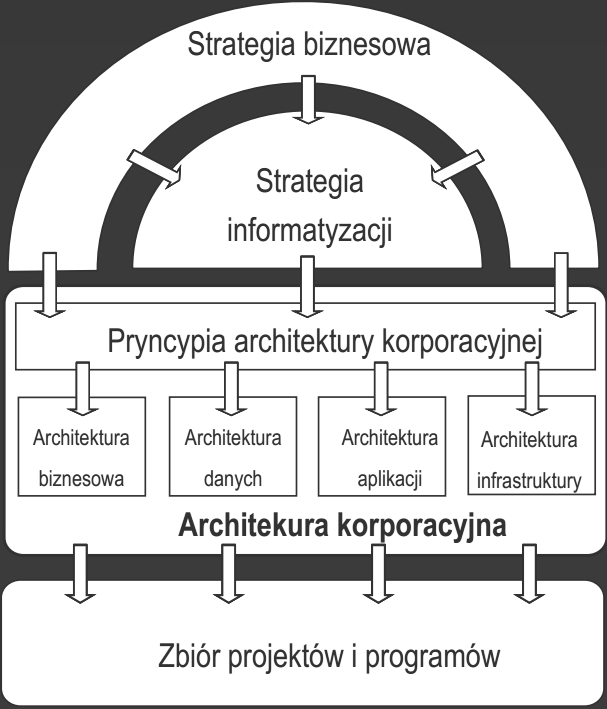
\includegraphics[width=8cm]{img/ea.png}
\caption[Umiejscowienie architektury w korporacji.]{Umiejscowienie architektury w korporacji. \cite{SOMAArsIBMJour}}\label{ea_arch}
\end{centering}
\end{figure}

W ostatnim czasie coraz bardziej popularnym terminem staje się \quotedblbase architektura korporacyjna IT\textquotedblright. Wykazuje ona pewne różnice w porównaniu do \quotedblbase zwykłej architektury korporacyjnej\textquotedblright. 

Jednym z elementów, które różnicują te dwa pojęcia jest cel opracowania architektury. Zwykła architektura korporacyjna nakierowana jest na zwiększenie efektywności działania w kontekście całej organizacji. Architektura korporacyjna IT kładzie zaś nacisk na zwiększenie efektywności działania IT w kontekście biznesowych potrzeb organizacji. 

Architektura korporacyjna stanowi szersze pojęcie pod względem zakresu opracowania architektury. Pojęcie to obejmuje organizację jako całość, natomiast architektura korporacyjna IT skupia się jedynie na obszarze IT danej jednostki. 

Istotnym elementem, o którym należy wspomnieć prowadząc rozważania na temat architektury korporacyjnej jest pojęcie \quotedblbase ładu architektonicznego \textquotedblright (ang. \emph{Enterprise architecture governance}). Stanowi on przede wszystkim mechanizm dostarczający struktury, za pomocą której jest ustanawiany zbiór celów tworzenia architektury korporacyjnej oraz środków, poprzez które możliwe osiąganie jest ich osiąganie i monitorowanie wydajności realizacji. 

Jego podstawowym celem w odniesieniu do systemów informatycznych jest zapewnienie zgodności podejmowanych decyzji z zakresu IT z opracowaną architekturą korporacyjną. 

Dobrze wprowadzony ład architektoniczny zapewni niezbędną dla organizacji elastyczność architektury korporacyjnej.

\section{Korzyści z wdrożenia architektury korporacyjnej}
Budowy architektury korporacyjnej nie powinno rozpatrywać się jedynie jako działania z obszaru informatyki, ale jako całościowego przedsięwzięcia z pogranicza zarządzania, jak i informatyki. Opracowanie architektury korporacyjnej nie należy rozważać jako cel sam w sobie, ale jako stan pośredni postrzegany jako narzędzie pomocnicze do wykonania określonych działań wewnątrz organizacji. Takie podejście może przynieść organizacji szereg korzyści
\begin{itemize}
\item{lepsze dopasowanie realizowanych rozwiązań informatycznych do potrzeb strategicznych danej organizacji,}
\item{zapewnienie większej interoperacyjności systemów informatycznych,}
\item{wykorzystywanie tych samych komponentów może spowodować znaczne obniżenie kosztów działań w zakresie wprowadzania architektury korporacyjnej,}
\item{możliwość szybszego podejmowania spójnych decyzji w zakresie tworzenia systemów informatycznych,}
\item{efektywniejsze koordynowanie z perspektywy dziań długoterminowych modyfikacji i rozbudowy poszczególnych systemów informatycznych,}
\item{ułatwienie zarządzania finansami przeznaczonymi na cele IT,}
\item{ułatwienie wdrożenia SOA,}
\item{automatyzacja, optymalizacja i przejrzystość procesów biznesowych - zdefiniowana architektura korporacyjna pozwala zidentyfikować wszystkie procesy, gdzie możliwa jest automatyzacja, wyeliminować dublujące się czynności pomiędzy procesami.}
\item{ograniczenie ryzyka operacyjnego - wdrażając architekturą korporacyjną można znacznie zmniejszyć ryzyko operacyjne, zarówno poprzez automatyzację procesów, jak i lepszą kontrolę operacji.}

Nie każda organizacja musi stosować sformalizowane podejście do zarządzania architekturą korporacyjną. Dużo zależy od złożoności organizacji - rozpatrywanej w ujęciu systemowym. Istotna jest również zmienność organizacji wynikająca na przykład ze zmienności otoczenia Im organizacja jest bardziej złożona i im bardziej podlega zmianom, tym stosowanie architektury korporacyjnej jest bardziej uzasadnione. \cite{ArchKorpSob}
\end{itemize}

\section{Podejście do budowy architektury korporacyjnej}
Budowa architektury korporacyjnej nie stanowi zadania trywialnego. Bardzo istotnym czynnikiem wpływającym na sukces jej wdrożenia do danej organizacji jest odpowiednie projektowanie i podejmowanie odpowiednich decyzji architektonicznych. 

Projektując architekturę korporacyjną należy rozważyć dwa główne problemy. Pierwszy dotyczy celu jej opracowywania. Przede wszystkim czy architektura korporacyjna ma mieć zastosowanie jako narzędzie wspierające określone przedsięwzięcie transformacyjne, czy też być na stałe wbudowana w ramy organizacji. Drugi problem związany jest z określeniem zakresu prac nad architekturą korporacyjną. Należy określić poszczególne wymiary: horyzont czasowy, zakres geograficzny organizacji oraz poziom szczegółowości w poszczególnych domenach. 

Opracowując architekturę korporacyjną można skorzystać z jednej dwóch ścieżek:
\begin{itemize}
\item{wychodząca od architektury dla stanu bazowego - polega na opracowaniu najpierw architektury dla stanu bazowego (\quotedblbase jak jest\textquotedblright) bezpośrednio w czterech domenach architektonicznych: aplikacji, danych, biznesowej i technicznej. W kolejnym kroku analizowane są luki we wszystkich wymienionych domenach oraz przygotowany jest plan przejścia (ang. \emph{roadmap}) pomiędzy stanem bazowym i docelowym. Do zalet tego podejścia można zaliczyć prostotę od strony zarządczej (można zidentyfikować i dobrze opisać poszczególne etapy prac). Wadę stanowi natomiast ryzyko zbyt dużego skupienia się na architekturze bazowej i wykonania analiz na zbyt dużym poziomie szczegółowości.}
\item{wychodząca od architektury biznesowej - opiera się na wykonaniu czterech kroków. W trzech pierwszych dla stanu bazowego \quotedblbase jak jest\textquotedblright, jak i dla stanu docelowego \quotedblbase jak będzie\textquotedblright opracowywane są kolejno architektury: biznesowa, danych i aplikacji oraz techniczna. W każdym z wymienionych kroków jest dokonywana również analiza luk. Mając opracowane architektury dla poszczególnych domen przygotowywana jest zbiorcza analiza luk oraz plan przejścia (ang. \emph{roadmap}) pomiędzy stanem bazowym i docelowym. Zaletą tej ścieżki jest dostarczenie na najwcześniejszym etapie kluczowego elementu architektury korporacynej - architektury biznesowej. Stanowi to dobrą podstawę dla opracowywania kolejnych architektur. Do wad podejścia zaliczyć można ryzyko z częstym występowaniem niskiego poziomu części biznesowej organizacji. \cite{ArchKorpSob}}
\end{itemize}

\section{SOA}
\subsection{Czym jest SOA?}
Trudno o jednoznaczną definicję SOA (ang. \emph{Service Oriented Architecture} – architektura zorientowana na usługi). Definicja SOA jest subiektywna, zależna od punktu widzenia. Z perspektywy biznesowej (odbiorcy usług) rozumieć ją można jako zestaw usług wspierających realizację procesów biznesowych. Odnosząc się do SOA z perspektywy IT widzimy ją jako infrastrukturę potrzebną do dostarczenia tych usług.
	
Organizacja W3C (World Wide Web Consortium) podjęła próbę zdefiniowania SOA. Według niej SOA to zbiór komponentów, które mogą być wywoływane, i których interfejsy mogą być publikowane i wykrywane (ang. \emph{A set of components which can be invoked, and whose interface descriptions can be published and discovered}).

Z kolei firma IBM definiuje SOA jako podejście do budowania systemów rozproszonych dostarczających funkcjonalność aplikacji w postaci usług, które mogą być udostępniane aplikacjom zewnętrznym lub innym usługom. \cite{PlatIntGor}

Istnieje również manifest SOA, który głosi, że orientacja na usługi kształtuje punkt widzenia na to co chcemy wykonać, a SOA stanowi typ architektury, który jest wynikiem takiej orientacji. (ang. Service orientation is a paradigim that frames what you do. Service-oriented architecture (SOA) is a type of architecture that results from applying service orientation). \cite{SOAManifestoOrg}

SOA sama w sobie nie jest jednakże żadną konkretną architekturą. Nie można jej traktować jako produkt lub tylko zbiór określonych rozwiązań technologicznych. SOA to przede wszystkim sposób myślenia – strategia, której naturalna realizacja jest reprezentowana przez usługi. \cite{SOAsdj102009,SOAwJBBC} SOA stanowi pewnego rodzaju paradygmat, który prowadzi do określonej architektury. \cite{SOAsdj102009} SOA reprezentuje przesunięcie w inżynierii oprogramowania i podnosi poziom abstrakcji, grupując wspólne działanie procesów biznesowych i wystawiając to jako usługę. \cite{CompSOAMet}
	
Mianem usługi w SOA określa się zbiór funkcjonalności pewnej aplikacji, który jest udostępniany jako interfejs. \cite{SOAawidptas} Organizacja OASIS definiuje usługę w SOA jako mechanizm udostępniający jedną lub więcej funkcji, do których dostęp jest zapewniany przez zalecany interfejs i wykonywany zgodnie z ograniczeniami i politykami określanymi przez opis usługi (ang. \emph{A mechanism to enable access to one or more capabilities, where the access is provided using a prescribed interface and is exercised consistent with constraints and policies as specified by the service description}). Operacje, zdefiniowane w interfejsie dostarczają funkcji biznesowych operując na obiektach biznesowych. Ponadto owe usługi są dostępne poprzez sieć.

\subsection{Historia SOA}
Przez ostatnie dekady tworzenie oprogramowania opierało się na kilku różnorodnych metodach. Jednym z ich podstawowych celów było radzenie sobie z coraz bardziej złożonym procesem wytwarzania oprogramowania. W ramach walki ze złożonością opracowano gruboziarniste konstrukcje takie jak funkcje, klasy i komponenty. Można myśleć o tych nich jak o \quotedblbase czarnych skrzynkach\textquotedblright (ang. \emph{Black boxes}). 

Te \quotedblbase czarne skrzynki\textquotedblright ukrywają swoje implementacje poprzez dostarczanie kontrolowanego dostępu do ich funkcjonalności poprzez interfejs. W pewnym momencie dostrzeżono, że ilość czarnych skrzynek jest zbyt duża. Problem ten rozwiązano grupując poszczególne \quotedblbase czarne skrzynki\textquotedblright w komponeenty. \cite{SteveMichSOA} 

Określenia \quotedblbase SOA\textquotedblright  lub \quotedblbase Architektura zorientowana na usługi\textquotedblright zostały po raz pierwszy wykorzystane w pracy naukowej analityka z firmy Garnter Yefim V. Natis w dniu 12 kwietnia 1996 roku. Wcześniej w 1994 roku Alexander Pasik stworzył istotne podstawy do zdefiniowania SOA. 

Przełomowym momentem w historii powstawania SOA było utworzenie usług typu \emph{Web Service} przez firmę Microsoft w 2000 roku. \cite{JosSOAHist}

\subsection{Budowa SOA}
SOA wprowadza nowe podejście do budowy i zarządzania infrastrukturą informatyczną. Adaptacja SOA wiąże się z reguły ze zmianami w wielu obszarach funkcjonowania firmy. Ściśle wiąże się z panującymi w niej procesami biznesowymi i wymaga odpowiedniego dostosowania.

Systemy opierające się na SOA składają się z zestawu aplikacji biznesowych (rys. \ref{PRZArchSOA}) pogrupowanych w niezależne komponenty, które komunikują się ze sobą wymieniając usługi. \cite{SOAwJBBC}. 

\begin{figure}[h!tbp]
\begin{centering}
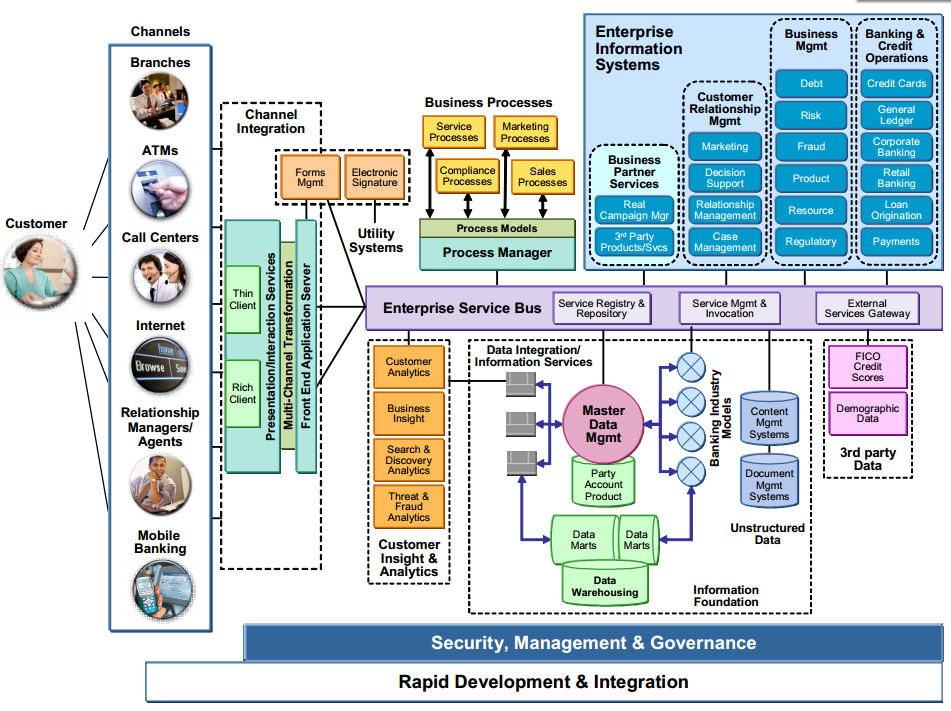
\includegraphics[width=15cm]{img/soa_arch.png}
\caption[Przykładowa architektura SOA.]{Przykładowa architektura SOA.}\label{PRZArchSOA}
\end{centering}
\end{figure}

Komponenty te można traktować jako tzw. „czarne skrzynki”. Klient korzystający z usługi otrzymuje jedynie interfejs. Implementacja udostępnionych metod nie jest dla niego istotna.
Rozwiązania stosowane w SOA pomagają zapanować nad złożonością systemu. Podstawowa budowa SOA opiera się z reguły na szynie ESB (ang. Enterprsie Service Bus) integrującej poszczególne usługi. ESB jest efektywnym środkiem komunikacji w SOA. Pomaga uwolnić się od sieci powiązań „każdy z każdym”. Odpowiada za przesyłanie komunikatów do odpowiednich komponentów. Rozbudowa systemu polega na dołączaniu nowych usług do szyny integracyjnej. 
	
Komunikaty zanim zostaną wysłane do punktu docelowego często poddawane są transformacjom i odpowiedniemu dostosowaniu za pomocą mediacji (ang. \emph{Mediations}) na ESB. Przetworzony komunikat odpowiada formie jakiej oczekuje dostawca usługi.
	
Rejestr SOA (ang. \emph{SOA registry}) stanowi centralny punkt informacyjny na temat sposobu dostępu, definicji, reguł, bezpieczeństwa i innych danych wymaganych do wykorzystania usług udostępnionych w danym środowisku SOA. Zawiera informacje gdzie poszczególne komponenty SOA są umieszczone. Na jego podstawie ESB potrafi prawidłowo przekierowywać żądanie usługi i ewentualną odpowiedź, a aplikacje i usługi korzystające z usług składowych potrafią skonstruować jej prawidłowe wywołanie.
	
Istotnym elementem w systemach typu SOA jest repozytorium (ang.\emph{SOA repository}). Stanowi ono centralny „magazyn” dla elementów składowych usług takich jak: kod źródłowy, zestawy instalacyjne, specyfikacja itp. Repozytorium usług jest tworzone i wykorzystywane głównie na etapie projektowania usług.

\subsection{Usługa sieciowa w SOA}
Usługa sieciowa w SOA (ang. \textit{Web Service}) stanowi usługę świadczoną przez sieć – na przykład Internet. Składnik oprogramowania niezależny od platformy sprzętowej oraz implementacji. Może być zdefiniowany za pomocą języka opisu usług – na przykład bazującym na XML WSDL (ang. Web Service Definition Language), publikowana i wyszukiwana w rejestrze (np. UDDI) oraz wywoływana zdalnie przez opisujący ją interfejs. 
Z reguły Web Service opiera się na konstrukcji uwzględniającej trzy typy komponentów (rys. \ref{WSArchFunc}) : klienta usługi (ang. service requestor), dostawcę usługi (ang. service provider) oraz rejestr usług (service registry) lub broker usług (ang. service broker).  Transport danych w przypadku Web Service z reguły opiera się na HTTP lub HTTPS z wykorzystaniem SOAP.

Każdy z komponentów jest odpowiedzialny za pełnienie swojej roli:
\begin{itemize}
\item{dostawca usługi tworzy i wdraża Web Service. Publikuje również dostępność opisanego za pomocą WSDL Web Service’u w rejestrze usług (lub brokerze usług),}
\item{rejestr usług lub broker usług odpowiada za rejestrację i kategoryzację opublikowanych usług. Dostarcza również możliwość ich wyszukiwania,} 
\item{klienci usług używają rejestru usług (lub brokera usług) do wykrycia Web Service’u opisanego za pomocą WSDL, a następnie wykonują zapytanie do dostawcy usługi. Dostawca usługi udziela odpowiedzi klientowi.}
\end{itemize}

\begin{figure}[h!tbp]
\begin{centering}
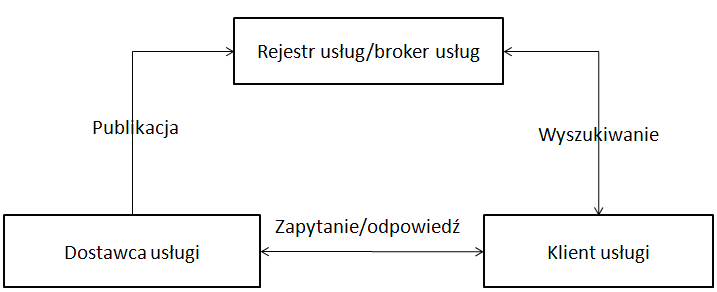
\includegraphics[width=11cm]{img/web_service.png}
\caption[Usługa sieciowa w SOA (Web Service).]{Usługa sieciowa w SOA (Web Service). \cite{AnRTeqq}}\label{WSArchFunc}
\end{centering}
\end{figure}

\subsection{Warstwy architektury SOA}
W SOA można wyszczególnić dziewięć warstw architektury. Każda z nich składa się z modelu fizycznego oraz logicznego. Model fizyczny opisuje sposób realizacji logiki za pomocą dostępnych technologii oraz produktów, natomiast logiczny zawiera wszystkie architektoniczne bloki, warunki logiczne, decyzje oraz inne - stanowi model konceptualny z dobranym poziomem abstrakcji.

Poszczególne warstwy w SOA to:
\begin{itemize}
\item{Warstwa aplikacji - w jej skład wchodzą wszystkie aplikacje działające w środowisku IT i mające na celu wspieranie działania przedsiębiorstwa. Do przykładów można zaliczyć: aplikacje Java Enterprise lub .NET, systemy transakcyjne, bazy danych oraz systemy ERP i CRM.}
\item{Warstwa komponentów - obejmuje składniki oprogramowania realizujące konkretne operacje usług Odpowiada za fizyczną implementację usługi oraz jej opis dostarczając elementy zgodne z SCA (ang. \textit{Service Component Architecture}) oraz specyfikacją SDO (ang. \textit{Service Data Objects}).}
\item{Warstwa usług - stanowi zbiór wszystkich usług zdefiniowanych za pomocą kontraktu pomiędzy dostawcą, a odbiorcą o sposobie dostarczenia usługi.}
\item{Warstwa procesów biznesowych - w tej fazie tworzona jest kompozycja wielu usług realizujących konkretne biznesowe przypadku użycia. Proces biznesowy składa się z przepływów realizujących dany cel biznesowy organizacji i zagregowanych usług.}
\item{Warstwa prezentacji - stanowi często wspólny interfejs dostępu do usług. Odpowiada za dostarczanie funkcji biznesowych dla klientów końcowych.}
\item{Warstwa integracji - kluczowy element architektury SOA. Jej podstawową funkcją jest zlecenie klientom usług i dostarczanie ich przez dostawców. Przepływ operacji jaki jest wykonywany w tej warstwie to: odbiór zlecenia od klienta, dostarczenie go do dystrybutora, a następnie dostarczenie do klienta.}
\item{Warstwa jakościowa - obejmuje monitorowanie procesów biznesowych odnoszących się do podstawowych wskaźników wydajności danej organizacji. Pełni obserwację pozostałych warstw i informuje o zdarzeniach niezgodnych z zakładanymi.}
\item{Warstwa Business Intelligence - stanowi podstawę do budowania rozwiązań Business Intelligence umożliwiających modelowanie danych analitycznych i eksploracje. W tej warstwie włączane są kluczowe zagadnienia związane z obiegiem informacji w przedsiębiorstwach.}
\item{Warstwa zarządzania - odnosi się do zarządzania wszystkimi elementami cyklu życiu SOA oraz wszystkich warstw architektury (ze szczególnym naciskiem na warstwę jakościową). Wykorzystuje kluczowe wskaźniki wydajności lub efektywności (KPI) do egzekwowania wymagań jakościowych i funkcjonalnych wyspecyfikowanych przez przedsiębiorstwo. \cite{PlatIntGor}}
\end{itemize}

\subsection{Podstawowe zasady SOA}
Systemy SOA mogą być bardzo różnorodne. SOA nie narzuca konkretnych technologii, a jej realizacja może odbywać się na wiele sposobów. Komunikacja między komponentami w SOA może wykorzystywać różne kanały komunikacji: WS, HTTP, HTTPS, LDAP, FTP, IMAP, JMS, RMI. Budowa systemu SOA może wykorzystywać szynę integracyjną ESB lub broker (można również łączyć wiele szyn ESB ze sobą lub łączyć broker’y z ESB). Mimo tej dużej dowolności istnieje zestaw zasad, na których powinien opierać się każdy system SOA.
\begin{itemize}
\item{luźne powiązania - powiązania odnoszą się do połączeń lub relacji między poszczególnymi elementami. Termin „luźne powiązania” (ang. \emph{Loose Coupling}) stanowi jeden z fundamentów SOA. \cite{SOAsdj102009} Odwołuje się do sposobu w jaki komponenty SOA współpracują ze sobą.  Zasada „luźnych powiązań” promuje niezależną konstrukcję i ewolucję usług. Każdy z komponentów może pracować autonomicznie wykonując określone czynności. Pracując razem, wymieniają między sobą komunikaty i mogą realizować to co jest zwykle możliwe przez duże, monolityczne aplikacje. „Luźne powiązania” pozwalają również na łatwą dekompozycję komponentów i wykorzystywanie ich do innych celów.}
\item{interoperacyjność (ang. \emph{Interoperability}) - opiera się na współpracy pomiędzy systemami. Zapewnienie interoperacyjności jest kolejną bardzo istotną zasadą, o której należy pamiętać tworząc systemy SOA. W miarę rozwoju poszczególnych systemów (np. poprzez dodawanie nowych komponentów) problem integracji staje się coraz trudniejszy do rozwiązania. Należy już na etapie projektowania ograniczać do minimum oraz wybierać odpowiednie protokoły, które dany system będzie obsługiwał. \cite{SOAsdj102009}}
\item{kompozycyjność - zasada kompozycyjności (ang. \emph{composability}) jest związana z zachowaniem odpowiednich relacji między komponentami. Systemy, które podążają za ta zasadą cechują się możliwością łączenia swoich komponentów w różne kombinacje w celu spełnienia postawionych wymagań. Umiejętność efektywnego komponowania usług z już istniejących jest kluczowym wymogiem dla osiągnięcia niektórych z podstawowych celów przy tworzeniu systemów opierających się na architekturze zorientowanej na usługi.}
\item{reużywalność - każda tworzona usługa powinna zachowywać zasadę reużywalności (ang. Reusability).  Opiera się ona na takim projektowaniu usług, aby była możliwość wielokrotnego jej wykorzystania do tworzenia kolejnych usług. \cite{SOAsdj102009}}
\item{kontraktowość usług - każda usługa powinna mieć zdefiniowany kontrakt (ang. \emph{Service contract}), który zawierany jest każdorazowo pomiędzy usługą, a jej konsumentem. Wyrażane są przez nie cele i możliwości danej usługi. W kontraktach znajdują się również opisy informacji oferowanych  i oczekiwanych przez usługi. [SOAinfoq10]}
\item{abstrakcyjność - zasada abstrakcji (ang. \emph{abstraction}) zakłada, że kontrakty usług mogą zawierać jedynie niezbędne informacje i mogą udostępniać jedynie te informacje, które są w nich zdefiniowane. Zasada ta podkreśla potrzebę ukrycia przez usługi tak wielu informacji jak to tylo możliwe. [SOAterlprD]}
\item{autonomiczność usług - autonomia usługi (ang. service autonomy) jest kolejnym paradygmatem projektowania systemów typu SOA. Termin ten odwołuje się do usług o podwyższonej niezależności od środowisk wykonawczych. [SOAsrvautoWCSS] Usługa powinna mieć możliwość podmiany środowiska wykonawczego z lekkiego prototypowego (ang. lightweight prototype) do pełnowymiarowego (ang. full-blown), w którym są już uruchomione inne usługi odwołujące do niej. Zgodnie z zasadą autonomii każda z usług może być wdrażana, wersjonowana i zarządzana niezależnie od innych. [SOAinfoq10]}
\item{wykrywalność usług - zasada wykrywalności usług (ang. services discoverability) polega na tym, że usługi powinny być opisywane za pomocą meta danych w takich sposób, aby były efektywnie wyszukiwane, przetwarzane i interpretowane zarówno w czasie projektowania jak i wykonywania. [SOAinfoq10, SOAsrvautoWCSS]}
\item{spójność i ziarnistość usług - interfejsy usług w systemach SOA powinny być tak zaprojektowane, aby wiązały tylko określony zbiór wymagań biznesowych. \cite{SOAsdj102009} Należy zadbać o optymalną ziarnistość interfejsów dla obsługiwanych typów i rozmiarów danych (ziarnistość danych wejściowych i wyjściowych), wartości biznesowej oraz funkcjonalności (domyślna i parametryzowana ziarnistość funkcjnonalności). [SOAdefgranaaImp]}
\item{bezstanowość usług - zasada bezstanowości usług (ang. Services statelessness) odwołuje się do minimalizacji użycia zasobów i ograniczania się do przechowywania i przetwarzania tylko absolutnie niezbędnych informacji.  [SOAsrvautoWCSS ] Usługa nie może być w stanie przetrzymywać informacji o wcześniejszych żądaniach klienta. Każda z informacji powinna być odizolowana od innych. Skuteczne stosowanie zasady bezstanowości może znacząco zwiększyć wydajność rozwiązania oraz zmniejszyć współbieżne działanie usług. \cite{SOAsdj102009}}
\item{enkapsulacja - enkapsulacja (ang. Encapsulation) stanowi jedną z podstawowych zasad poprawnego projektowania systemów typu SOA. Zapewnienie odpowiedniej hermetyzacji dla usług sprowadza się do ukrywania szczegółów konfiguracyjnych oraz implementacyjnych danej usługi.}
\end{itemize}

\subsection{Korporacyjna szyna usług - ESB}
ESB (ang. \textit{Enterprise Service Bus}) stanowi abstrakcyjną warstwę wymiany komunikatów. W systemie informatycznym wprowadza znaczną elastyczność, ponieważ pozwala na dynamiczne przyłączanie i odłączanie usług. \cite{PlatIntGor}

Głównym celem korporacyjnej szyny usług jest dostarczanie pewnego rodzaju wirtualizacji dla korporacyjnych zasobów pozwalając na rozwijanie logiki biznesowej niezależnie od infrastruktury lub sieci oraz bez potrzeby pisania dodatkowego kodu. Zasoby w ESB są modelowane jako usługi, które oferują jedną lub więcej operacji biznesowych. \cite{IBMRBSoaPat}

Dobra praktyka projektowania architektury systemu zapewnia, że wszystkie połączenia między aplikacjami będą realizowane z wykorzystaniem szyny. \cite{PlatIntGor} Pełne sprostanie różnorodności wzorców integracji jakie oferuje SOA wymaga utrzymywania przez ESB trzech głównych paradygmatów integracji aplikacji korporacyjnych:
\begin{itemize}
\item{Architektura zorientowana na usługi - rozproszone aplikacje zbudowane są z ziarnistych usług wieleokrotnego użytku z dobrze zdefiniowanymi, opublikowanymi i zgodnymi ze standardami interfejsami.}
\item{Architektura zorientowana na komunikaty (ang. \textit{message-driven architecture}) - aplikacje wysyłają komunikaty między sobą.}
\item{Architektura zorientowana na zdarzenia (ang. \textit{event-driven architecture}) - aplikacje generują i konsumują usługi niezależnie od pozostałych.} \cite{IBMRBSoaPat}
\end{itemize}

Stosowanie szyny integracyjnej wiąże się z wieloma zaletami. Przede wszystkim powoduje zmniejszenie kosztów dzięki szybkiemu i elastycznemu rozwiązaniu integracji eliminującym połączenia typu \textit{point-to-point}. ESB umożliwia również rozwój obecnych środowisk bez wpływu na obecne co pozwala na łatwe rozszerzanie systemu o nowe funkcjonalności. \cite{IBMRBSoaPat}

\section{Adaptacja SOA w architekturze korporacyjnej}
Termin \emph{Enterprise SOA} jest bardzo popularny w ostatnich czasach. Wywodzi się z bardzo szerokiego zakresu. Posiada duże możliwości do łączenia elementów technologii z biznesem, jak i specyfikowania operacji poszczególnej usługi oferowanej pomiędzy systemami. Stanowi to również jedną z największych zalet SOA. \cite{EntSOACoryCanSoaML}

Architektura korporacyjna powinna dążyć do zapewnienia możliwie jak największej interoperacyjności tworzonych rozwiązań informatycznych i jak najłatwiejszej ich integracji. Problemem jest jednak zacieranie się świata biznesu i IT w kontekście architektury korporacyjnej.

W rozwiązaniu tych problemów pomaga SOA, która opiera się na koncepcji usług, kontraktów, procesów oraz orkiestracji (ang. \emph{orchestration}). Wszystkie z wymienionych elementów są powiązane z domeną biznesową. Pozwalają na kompleksowe opisywanie krytycznych dla biznesu funkcjonalności. 

Problem ze względu na swój zakres oraz ilość elementów branych pod uwagę do jego rozwiązania jest stosunkowo złożony. Konieczne jest dlatego oparcie się na odpowiedniej metodyce. W pracy zostanie przedstawione jak zaadaptować SOA w architekturze korporacyjnej z wykorzystaniem SoaML z wykorzystaniem opracowanej optymalnej metody.

\chapter{Przegląd języków do projektowania systemów informatycznych o architekturze SOA}

\section{Wstęp}
Modele tworzone w ramach architektury korporacyjnej możemy traktować na kilka sposobów:
\begin{itemize}
\item{medium komunikacyjne między interesariuszami, którzy reprezentują zarówno dział informatyki, jak i inne jednostki organizacji;}
\item{forma ukazania i dokumentowania pewnych decyzji - zarówno na poziomie technicznym w ramach architektury infrastruktury technicznej (na przykład w zakresie dotyczącym serwerów oraz sieci komputerowych), jak i biznesowym w ramach architektury biznesowej (odnośnie przebiegu procesów biznesowych).}
\item{abstrakcja organizacji, opisująca strukturę i działanie poszczególnych elementów składowych (zarówno na płaszczyźnie technicznej, jak i biznesowej). Taki opis pozwala na planowanie rozwoju organizacji, wspomaga jej transformację.}
\end{itemize}

Opracowana architektura powinna być zrozumiała dla odbiorcy, tak aby na jej podstawie można było podjąć określone decyzje związane z funkcjonowaniem organizacji lub wdrożeniem określonych rozwiązań informatycznych. Należy wziąć również pod uwagę fakt, że potencjalnymi osobami często mogą być różne osoby - analityk systemowy, projektant systemów, czy też osobą odpowiedzialną za komórkę informatyczną w danej organizacji). \cite{ArchKorpSob}

W niniejszym rozdziale zostaną omówione języki wykorzystywane do modelowania architektury korporacyjnej. Przy wykorzystaniu SoaML lub ArchiMate można w pełni zamodelować architekturę korporacyjną. Inne jęzki jak: BPEL, BPMN, czy UML, mogą wspierać proces projektowania jedynie w poszczególnych domenach.

\section{SoaML}
\subsection{Czym jest SoaML?}
SoaML (\emph{The Service oriented architecture Modeling Language}) stanowi język wyspecyfikowany przez OMG (\emph{Object Managment Group}) w 2009 roku, który definiuje profil UML i metamodel dla projektowania usług w architekturze zorientowanej usługowo. Podstawowym celem SoaML jest modelowanie i projektowanie usług, tak aby wspierać dewelopment oparty na podejściu sterowanym modelami z perspektywy biznesowej i IT.

SoaML definiuje trzy różne podejścia dla specyfikowania usług: 
\begin{itemize}
\item{Proste interfejsy (ang. \emph{Simple interfaces}) - prosty interfejs, który opiera się na jednokierunkowej interakcji dostarczanej przez uczestnika interakcji jako interfejs UML. Uczestnik otrzymuje operacje na swój port i może dostarczyć rezultaty dla wywołującego zapytanie. Ten rodzaj jednokierunkowej interakcji może być stosowany dla anonimowych inicjatorów interakcji. Uczestnik interakcji nie ma informacji o inicjatorze ani o  porządku usług. Jednokierunkowe usługi są najczęściej określane jako \quotedblbase RPC style Web Services\textquotedblright. Prosty interfejs wykorzystywany jako port usługi może opcjonalnie stanowić element \emph{ServiceInterface}.} \cite{SOAMLOMG}

\begin{figure}[h!tbp]
\begin{centering}
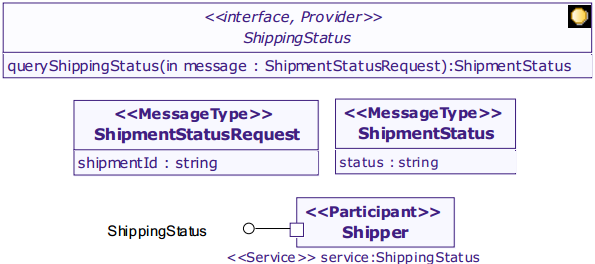
\includegraphics[width=11cm]{img/simple_interface_based_approach.png}
\caption[Specyfikacja usługi \emph{Ship Status} wykorzystując podejście \quotedblbase prostego interfejsu\textquotedblright. Zawiera prosty interfejs dostawcy usługi, jego operacje, typy wiadomości i odpowiedni port uczestnika interakcji.]{Specyfikacja usługi \emph{Ship Status} wykorzystując podejście \quotedblbase prostego interfejsu\textquotedblright. Zawiera prosty interfejs dostawcy usługi, jego operacje, typy wiadomości i odpowiedni port uczestnika interakcji. \cite{SoaMLErvBase}}\label{simple_interface_based_approach}
\end{centering}
\end{figure}

\item{Interfejsy usług (ang. \emph{Service interfaces}) - podejście bazujące na interfejsach usług skupia się na dwu i większej ilości interakcji między usługami, wymagając jednocześnie wyspecyfikowania zbioru powiązanych ze sobą interfejsów w ramach specyfikacji jednej usługi. Opiera się na komponentach i zezwala na połączenia między nimi z wykorzystaniem portów. Porty powinny specyfikować pożądane i dostarczane interfejsy. 
\begin{figure}[h!tbp]
\begin{centering}
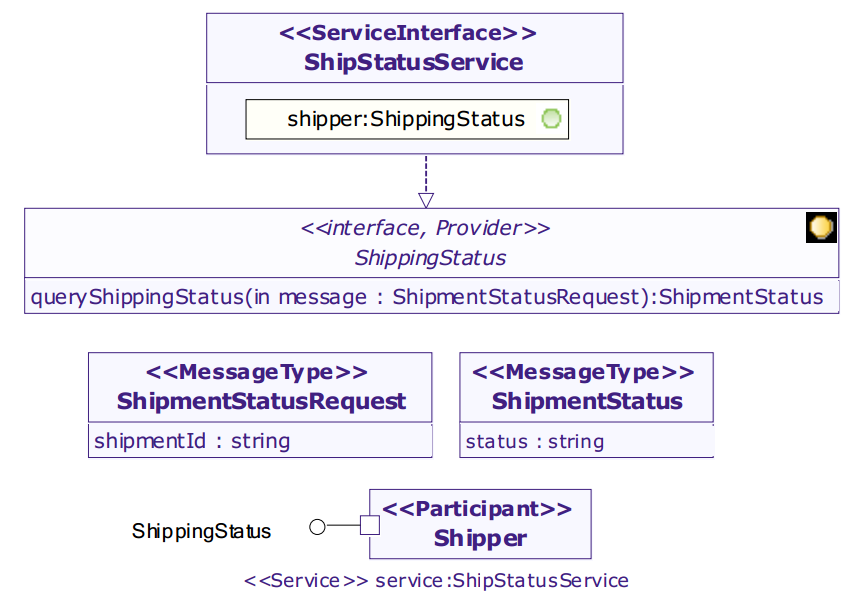
\includegraphics[width=11cm]{img/service_interface_based_approach.png}
\caption[Specyfikacja usługi \emph{ShipStatusService} wykorzystując podejście oparte na interfejsach usług.]{Specyfikacja usługi \emph{ShipStatusService} wykorzystując podejście oparte na interfejsach usług. \cite{SoaMLErvBase}}\label{service_interface_based_approach}
\end{centering}
\end{figure}} 

\item{Kontrakty usług (ang. \emph{contract interfaces}) - podejście w oparciu o kontrakty usług definiuje specyfikacje usług, które definiują role każdego uczestnika usługi (takich jak dostawców i klientów) oraz jakie interfejsy powinni implementować do realizacji ich ról w usłudze. Te interfejsy z kolei są typami portów uczestników, które zobowiązują ich do realizacji ról w danym kontrakcie usługi. Podejście to rozszerza elementy współpracy (ang. \emph{Collaboration}) UML do modelowania części strukturalnej interakcji usług. 
\begin{figure}[h!tbp]
\begin{centering}
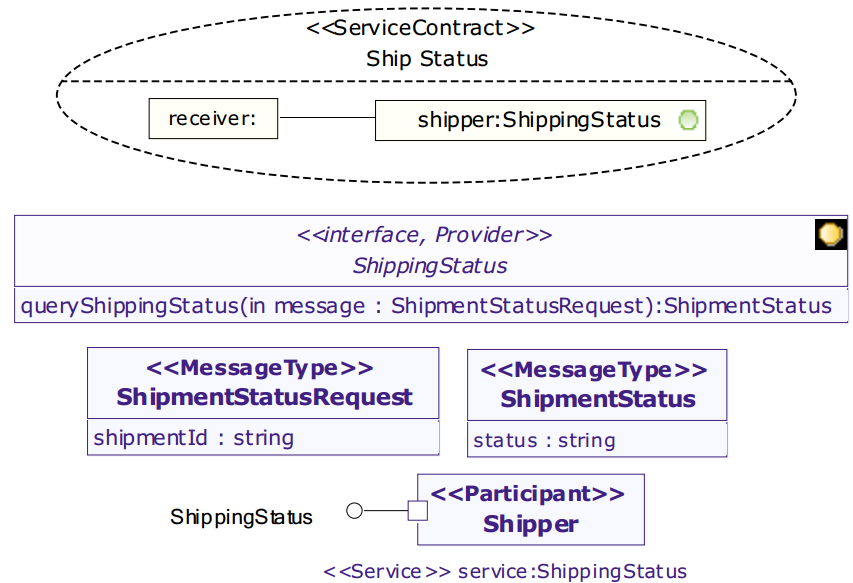
\includegraphics[width=11cm]{img/service_contract_based_approach.png}
\caption[Specyfikacja usługi \emph{Ship Status} wykorzystując podejście oparte na \quotedblbase kontrakcie usługi\textquotedblright. ]{Specyfikacja usługi \emph{Ship Status} wykorzystując podejście oparte na \quotedblbase kontrakcie usługi\textquotedblright. \cite{SoaMLErvBase}}\label{service_contract_based_approach}
\end{centering}
\end{figure}
}
\end{itemize}

Wszystkie podejścia charakteryzują się wykorzystywaniem różnych elementów UML. Podstawowa różnica pomiędzy podejściem bazującym na kontrakcie i interfejsie polega na zdefiniowaniu interakcji pomiędzy uczestnikami niezależnie od nich w \emph{ServiceContract}). Element ten określa obowiązki wszystkich uczestników interakcji lub indywidualnie dla każdego z uczestników i zapytań. 

\subsection{Modelowanie z wykorzystaniem SoaML}
SoaML wspiera modelowanie wymagań dla SOA w oparciu o specyfikowanie usług systemowych, indywidualnych usług dla interfejsów oraz specyfikację implementacji usług. Metamodel SoaML \cite{soaml_metamodel} rozszerza metamodel UML dla bezpośredniego modelowania usług w rozproszonych środowiskach. \cite{SoaMLErvBase}

\begin{figure}[h!tbp]
\begin{centering}
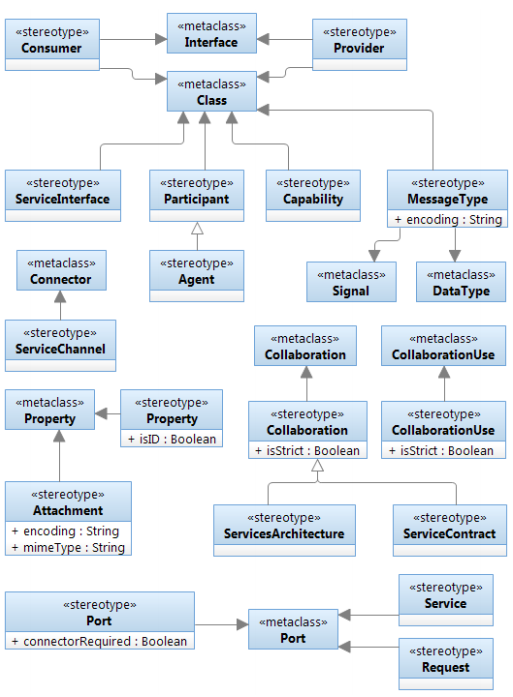
\includegraphics[width=11cm]{img/soaml_metamodel.png}
\caption[Podstawowe rozszerzenia UML zdefiniowane jako stereotypy dla SoaML.]{Podstawowe rozszerzenia UML zdefiniowane jako stereotypy dla SoaML. \cite{SoaMLErvBase}}\label{soaml_metamodel}
\end{centering}
\end{figure}

SoaML charakteryzuje się dodatkowymi abstrakcjami \cite{PlatIntGor} i rozszerza UML w sześciu głównych obszarach: 
\begin{itemize}
\item{Uczestnicy realizujący kontrakty (ang. \emph{Participants}) - na diagramach SoaML oznaczeni są stereotypem \emph{<<Paricipant>>}.}
\item{Interfejsy usług (ang. \emph{Service interfaces}) - wykorzystywane do opisywania operacji dostarczanych i wymaganych do pełnej funkcjonalności usługi. Interfejs usługi może być wykorzystywany jako protokół dla portu usługi lub odpytywany port. Oznaczone są stereotypami \emph{<<ServiceInterface>>}.}
\item{Kontrakty usług (ang. \emph{Service contracts}) - wykorzystywane do opisywania wzorców interakcji między encjami usług. Umowa o świadczenie usług jest używana do modelowania porozumienia między dwiema lub większą ilością stron. Każda z usług z kontraktu posiada interfejs, który reprezentuje ją jako dostawcę bądź konsumenta. Oznaczone są stereotypami \emph{ServiceContract}}
\item{Usługi architektur (ang. \emph{Services architecture}) - wyższy element widoku prezentujący zbiór elementów SOA. Oznaczany stereotypem <<ServicesArchitecture>>}
\item{Dane usług (ang. \emph{Service data}) - wykorzystywane do opisywania komunikatów dla usług i ich załączników. Element \quotedblbase Typ wiadomości\textquotedblright} (ang. \emph{Message Type}) jest używany do specyfikowania informacji wymienianych pomiędzy konsumentami usług i dostawcami. Określa rodzaj komunikatu. Oznaczany jest na diagramach jako stereotyp \emph{<<MessageType>>}. Załączniki są oznaczane jako stereotyp \emph{<<Attachment>>.}
\item{Funkcjonalność (ang. \emph{Capabilities}) - kolejny zdefiniowany element SoaML. Na diagramach klas określa funkcjonalność lub zasoby jakie oferują uczestnicy architektury. Przedstawiany jest w postaci komponentu ze stereotypem \emph{capabilities}. \cite{SoaMLErvBase}}
\end{itemize} 


\section{ArchiMate}
\subsection{Czym jest ArchiMate?}
ArchiMate stanowi otwarty i niezależny język modelowania dla architektur korporacyjnych. Zapewnia instrumenty, aby umożliwić architektom przedsiębiorstwa opis, analizę i wizualizację relacji między domenami biznesu w jednoznaczny sposób. Pozwala ponadto na opisywanie procesów biznesowych, struktur organizacyjnych, przepływów informacji, systemów informatycznych oraz technicznej infrastruktury.

ArchiMate to techniczny standard The Open Group. Jest wspierany przez różne narzędzia informatyczne do modelowania architektury korporacyjnej jak na przykład: Enterprise Architect, BizzDesign Architect, ARIS lub Microsoft Visio. \cite{OpenGrArch} 

ArchiMate bazuje na dwóch podstawowych założeniach:
\begin{itemize}
\item{podejściu warstwowym - związane z warstwą biznesową, aplikacji, danych i techniczną;}
\item{podejściu zorientowanym na usługi - usługi zewnętrzne są udostępniane przez warstwę niższą i wykorzystywane przez warstwę wyższą (na przykład warstwa aplikacji udostępnia usługi wykorzystywane w ramach warstwy biznesowej). ArchiMate wprowadza ponadto pojęcie usług wewnętrznych, które są wykorzystywane w ramach określonej warstwy.}
\end{itemize}

Komunikacja pomiędzy warstwami: biznesową, aplikacyjną i technologiczną stanowi jedną z największych zalet ArchiMate.

W warstwie biznesowej (ang. \emph{Business layer}) zawarte są usługi świadczone klientom zewnętrznym oraz produkty. Są one realizowane przez przez procesy biznesowe i związanych z nimi aktorów biznesowych.

Warstwa aplikacji (ang. \emph{Application layer}) wspiera warstwę biznesową poprzez usługi aplikacyjne, które są realizowane przez poszczególne komponenty aplikacyjne.

Warstwa technologiczna (ang. \emph{Technology layer}) odzwierciedla usługi infrastrukturalne (na przykład usługi komunikacyjne), niezbędne do działania aplikacji.

Od wersji 2.0 możliwości języka ArchiMate zostały rozbudowane poprzez zdefiniowanie części centralnej oraz rozszerzeń związanych z motywacją, implementacją i konfiguracją. \cite{ArchKorpSob}


\subsection{Modelowanie z wykorzystaniem ArchiMate}
Jednym z najbardziej popularnych podejść do modelowania architektury korporacyjnej z wykorzystaniem ArchiMate jest oparcie się na metodzie \emph{top-down}. 

W początkowym etapie powinno zdefiniować się warstwę biznesową. Zalecane jest dlatego utworzenie najpierw \emph{Business Model Canvas}. Stanowi on szablon dla dokumentowania nowych lub istniejących modeli biznesowych. W efekcie zostaje utworzony diagram złożony z bloków opisujących różne istotne elementy organizacji. Stanowi on szkic strategii, który ma zostać wdrożony w ramach struktur, procesów i organizacji. Składają się na niego takie elementy jak: segmenty klientów, propozycje wartości, kanały, relacje z klientami, strumienie przychodów, kluczowe zasoby, działania, partnerzy oraz struktura kosztów. 

Następnie powinno zidentyfikować się przepływy pomiędzy różnymi encjami \emph{Business Model Canvas} oraz dokonać mapowania ogólnego modelu biznesu jako usług powiązanych. W ArchiMate, na najwyższym poziomie, organizacja i odpowiadający jej model biznesowy może być reprezentowany jak pojedyncza usługa biznesowa (ang. \emph{Business Service}). Segmenty klientów i kluczowi partnerzy mogą być reprezentowani jako encje aktorów biznesowych (ang. \emph{Business actors}). Każdy z nich powinien mieć przypisaną co najmniej jedną rolę biznesową (ang. \emph{Business role}) i być połączonym z usługą organizacji przez biznesowe relacje interfejsu (ang. \emph{Business interface relationships}).

W kolejnym kroku rozwijane są szczegóły ogólnego modelu biznesowego. Następuje przejście z \emph{Business Model Canvas} na \emph{Enterprise Canvas}. 


\section{Inne języki}

\subsection{BPMN}
BPMN (ang. \textit{Business Process Modelling Notation}) stanowi standard modelowania procesów biznesowych opracowany przez Business Process Management Initiative (BPMI), a następnie rozwijany przez Object Management Group (OMG). 

Nie jest to język, który pozwoli na pełne zamodelowanie SOA lub architektury korporacyjnej. Można go wykorzystać jednak do modelowania fragmentu dotyczącego procesów biznesowych.

Definiuje diagramy nazywane diagramami procesu biznesowego - zaprojektowane tak, żeby z jednej strony były łatwe do zrozumienia, a z drugiej pozwalały na modelowanie również złożonych procesów. Składa się ze skończonego i jednoznacznie zdefiniowanego zbioru elementów graficznych. Pozwalają na budowanie zarówno modeli procesów zrozumiałe przez analityków biznesowych, jak również przez kadrę zarządzającą.

Elementarne typy obiektów BPMN stanowią: 
\begin{itemize}
\item{obiekty przepływu (ang. \emph{Flow objects}) - stanowią je elementy odnoszące się do zdarzeń, czynności lub obiektów decyzyjnych}, 
\item{obiekty łączące (ang. \emph{Connecting objects})} - do tej grupy zaliczyć można sekwnecje elementów, komunikaty, 
\item{tory przepływu (ang. \emph{Swimlanes})},
\item{artefakty (ang. \emph{Artifact})}.
\end{itemize}

BPMN może być wykorzystywany do modelowania:
\begin{itemize}
\item{procesów interakcji (globalnych) - wykorzystywane do reprezentacji interakcji między dwoma lub większą ilością obiektów biznesowych,}
\item{abstrakcyjnych procesów (publicznych) - reprezentują interakcje między procesami prywatnymi a uczestnikami zewnętrznymi, albo dwoma procesami prywatnymi,}
\item{prywatnych procesów biznesowych - procesy wewnętrzne, specyficzne dla konkretnej interakcji.}
\end{itemize}

\subsection{BPEL}
BPEL (Business Process Execution Language) stanowi język pozwalający na definiowanie i wykonywanie procesów biznesowych. Został opracowany przez konsorcjum OASIS.

Podobnie jak BPMN pozwala na modelowanie jedynie fragmentu architektury korporacyjnej związanej z procesami biznesowymi. Jest postrzegany jako procesowe rozszerzenie standardów zdefiniowanych dla usług sieciowych, które pozwalają na współpracę między aplikacjami w środowiskach heterogenicznych. Opiera się na takich standardach jak SOAP, WSDL oraz Universal Description, Discovery and Integraton (UDDI). 

W BPEL można opisywać procesy na dwa sposoby - abstrakcyjny lub wykonywalny.

Proces abstrakcyjny jest określony tylko częściowo. Musi być otwarcie zadeklarowany jako abstrakcyjny i nie powinien być wykonywalny. Ponadto  udostępnia dwa mechanizmy umożliwiające ukrycie jego szczegółów: nieprzezroczyste (ang. \emph{opague tokens}) oraz pominięcie (ang. \emph{omission}).

Z kolei proces wykonywalny w pełni specyfikuje opis, który można umieścić w środowisku wykonawczym. Musi być w pełni zdefiniowany wyłącznie na podstawie usług sieciowych oraz danych przedstawionych w języku XML. Konstrukcje procesu wykonywalnego powinny być dostępne dla procesu abstrakcyjnego. 

Istnieją również rozszerzenia języka BPEL. Jednym z nich jest BPEL4WS, który nie uwzględnia człowieka w procesie biznesowym. Przeciwieństwo stanowi zaś BPEL4People, w którym człowiek stanowi część procesu biznesowego. Innym przykładem jest jeszcze BPELJ, który umożliwia zastąpienie usług sieciowych małymi aplikacjami napisanymi na podstawie języka Java. \cite{PlatIntGor}

\subsection{UML}
UML (Unified Modeling Language) jest jednym z najpowszechniejszych graficznych języków wykorzystywanych do modelowania architektury korporacyjnej. Został stworzony w 1994 roku i rozwijany jest w ramach OMG (Object Management Group). 

Przy wykorzystaniu elementów języka UML można wizualizować, specyfikować oraz budować systemy informatyczne. Stosowanie UML pozwala w graficzny sposób odwzorować zarówno behawioralne jak i strukturalne spojrzenia na system.

Modelowanie systemów z wykorzystaniem UML umożliwia jednoczesne dokumentowanie całości systemu w zrozumiały dla całego zespołu sposób. \cite{PlatIntGor} UML służy głównie do modelowania systemów informatycznych, w tym również uwzględniających aspekty architektoniczne. 

UML znajduje coraz częściej zastosowanie w inżynierii systemów, do  modelowania procesów biznesowych lub reprezentacji struktur organizacyjnych. W tym celu bardzo często wykorzystywane są możliwości jego rozszerzenia - na przykład za pomocą profili. Istotą ich stosowania jest fakt, że dodajemy możliwość używania konkretnych znaczeń w stosunku do istniejących elementów modelu.


\subsection{IDEF}
Języki IDEF (Integrated DEFinition Methods) stanowią rodzinę języków wykorzystywaną do analizy biznesowej i modelowania. Pierwotnie wiązane były głównie z wojskowością.  Obecnie IDEF ma bardzo szerokie zastosowania i występuje w wielu odmianach.

IDEF0 są wykorzystywane do modelowania funkcji. Pozwalają na modelowanie decyzji, działań i czynności. Zarówno na poziomie systemu informatycznego, jak i całej organizacji. Celem opracowania IDEF0 było utworzenie języka pozwalającego na ułatwienie analizy systemów i organizacji, a także poprawienie komunikacji pomiędzy analitykami biznesowymi i ich klientami. 

IDEF3 pozwala na modelowanie procesów biznesowych. Przystosowany jest również do prezentowania behawioralnych aspektów planowanych lub działających systemów. 

IDEFIX został utworzony z kolei z przeznaczeniem modelowania danych. Dostarcza semantycznych konstrukcji, które pozwalają na modelowanie konceptualnych schematów dla struktur danych używanych na poziomie całej organizacji.

\chapter{Metody projektowania rozwiązań w architekturze usługowej}

\section{Wstęp}

\section{RUP4SOA}
\subsection{Czym jest RUP?}
RUP (ang. \textit{Rational Unified Process}) stanowi proces  wytwarzania oprogramowania oparty na iteracjach. Metoda ta została zdefiniowana przez grupę Rational Software (przejętą przez firmę IBM w roku 2003). 

RUP zapewnia zdyscyplinowane podejście do przydzielania zadań i obowiązków w ramach rozwoju organizacji. Celem podstawowym tej metody jest dostarczenie wysokiej jakości oprogramowania spełniającego potrzeby użytkowników końcowych w zgodzie z harmonogramem i ramami budżetowymi. \cite{RUPIntRat} Stanowi przede wszystkim bardzo duży zbiór praktyk, który może być dostosowywany i rozszerzany w celu jak najlepszego dopasowania się do danej organizacji. Charaktertystyczne dla metody jest rozwój sterowany przypadkami użycia (ang. \textit{Use Case Driven Development}). \cite{RUPMartFow}

W RUP można wyróżnić poszczególne fazy:
\begin{itemize}
\item{faza początkowa (ang. \textit{inception}) – wstępne określenie wymagań, ryzyka, kosztu, harmonogramu, a także architektury systemu,}
\item{faza opracowania (ang. \textit{elaboration}) – ustalenie wymagań (większości przypadków użycia), architektury systemu oraz planu całego procesu wytwarzania systemu,}
\item{faza konstrukcji (ang. \textit{construction}) – tworzenie systemu (kolejnych komponentów), w trakcie następuje oddanie pierwszej (i być może dalszych) wersji użytkownikowi,}
\item{faza przekazania (ang. \textit{transiation}) – system jest przekazywany użytkownikowi, wdrażany, szkoleni są pracownicy obsługi systemu, następuje walidacja i końcowe sprawdzenie jakości.} \cite{RUPIntRat}
\end{itemize}
\subsection{Wykorzystanie RUP w projektowaniu SOA}
RUP4SOA stanowi modyfikację metody RUP i dołączono do niej zadania i produkty potrzebne przy projektowaniu rozwiązań w architekturze usługowej. RUP4SOA stanowi komercyjny plug-in dla framework'a RUP. Rozszerza standardowy pakiet o zbiór dodatkowych artefaktów i właściwości. W odróżnieniu od klasycznego RUP, metoda ta opiera się na wyróżnieniu trzech dyscyplin związanych z analizą i projektowaniem:
\begin{itemize}
\item{analiza i projektowanie architektury SOA - przygotowanie architektury SOA zgodnie z wymaganiami,}
\item{analiza i projektowanie kontraktów w architekturze SOA - analizie poddane są procesy integracyjne, związane z dostarczaniem usług i realizacją kontraktów między organizacjami,}
\item{analiza i projektowanie logiki usług SOA - identyfikacja usług w systemach informatycznych w jednostkach, w których wdrażana będzie architektura SOA}
\end{itemize}
Reszta dyscyplin jest analogiczna do metody RUP. \cite{PlatIntGor} W RUP4SOA można wyróżnić poszczególne fazy:
\begin{itemize}
\item {modelowanie biznesowe,}
\item {specyfikacja wymagań,}
\item {analiza i projektowanie architektury SOA,}
\item {analiza i projektowanie kontraktow SOA,}
\item {analiza i projektowanie logiki usług,}
\item {implementacja,}
\item {testowanie,}
\item {wdrożenie,}
\item {zarządzanie zmianą i konfiguracją,}
\item {zarządzanie projektem,}
\item {środowisko.}
\end{itemize}

W fazie analizy i projektowania przygotowywana jest architektura SOA zgodnie z postawionymi wymaganiami i modelem biznesowym. Istotne jest, aby opracowywana architektura była projektowana z zamysłem o jak najprostszej realizacji i późniejszym wdrożeniu. Kolejną dyscyplinę stanowi analiza i projektowanie kontraktów w architekturze usługowej. Ta faza opiera się na analizie procesów integracyjnych związanych z dostarczaniem usług i wymianą kontraktów między organizacjami. Następny element metody RUP4SOA stanowi analiza i projektowanie logiki usług SOA, który powiązany jest z identyfikacją usług informatycznych w organizacjach. 

Po fazach analizy i projektowania następują kolejno implementacja oraz testy. W następnym etapie utworzony produkt zostaje wdrożony na przygotowane środowisko. Równolegle trwają również prace związane z zarządzaniem projektem, konfiguracją oraz zmianami. \cite{PlatIntGor}

Podstwowym produktem wytworzonym przez Architekta oprogramowania w przypadku RUP4SOA jest model usług. Do podstawowych zadań Architekta oprogramowania zalicza się realizację fazy \quotedblbase identyfikacji usług\textquotedblright.

Projektant w RUP4SOA odpowiada za przygotowanie projektu usługi, a jego odpowiedzialność jest związana z produktami: komunikat, usługa, kanał usługi, bramka usługi, współpraca usługi, partycja usługi, specyfikacja usługi oraz komponent usługi. 

\subsection{Zalety i wady RUP4SOA}
RUP4SOA jest jedną z najpopularniejszych metod stosowanych do projektowania architektury usługowej. Największy nacisk kładzie na fazy związane z analizą i projektowaniem systemu informatycznego - rozszerzonym o elementy związane z usługami sieciowymi. Fakt ten może powodować większą zgodność między wyobrażnieniami klienta, a rzeczywistym produktem w formie systemu. 

Jedną z jej największych zalet jest również opieranie się na metodyce RUP, która wykorzystuje doświadczenia i praktyki przyjęte przez organizacje na przestrzeni wielu lat. \cite{JonSimRUPSoa}

Metoda ta nie specyfikuje wielu elementów istotnych do budowy rozwiązań integracyjnych. Skupia się na projektowaniu pojedynczego systemu, który może być jedynie włączony do platformy integracyjnej. \cite{PlatIntGor}

\section{SOMA}
\subsection{Czym jest SOMA?}
SOMA (ang. \textit{Servie-Oriented Modeling and Architecture} stanowi kolejną metodę projektowania systemów w architekturze usługowej. \cite{PlatIntGor} Metoda cyklu rozwoju oprogramowania definiująca kluczowe techniki i opisująca poszczególne role w projekcie SOA oraz struktury podziału pracy (WBS - ang. \textit{Work Breakdown Structure}). WBS obejmuje zadania związane z wejściowymi i wyjściowymi produktami pracy, z normatywnymi wskazówkami do szczegółowej analizy, projektowaniem, implementacją i wdrażaniem usług oraz komponentów potrzebnych do budowy wydajnego, reużywalnego środowiska.

SOMA została utworzona i jest rozwijana przez firmę IBM. W swoim podejściu metoda wykorzystuje wiele elementów z Worldwide Project Management Method (jedna z metod zarządzania projektami). \cite{SOMAArsIBMJour}

\subsection{Fazy metody SOMA}
SOMA bazuje na siedmiu podstawowych fazach:
\begin{itemize}
\item{modelowanie biznesowe (ang. \textit{business modeling and transformation}),}
\item{zarządzanie rozwiązaniem (ang. \textit{solution management}),}
\item{identyfikacja (ang. \textit{identification}),}
\item{specyfikacja (ang. \textit{specification}),}
\item{realizacja (ang. \textit{realization}),}
\item{implementacja (ang. \textit{implementation}),}
\item{monitorowanie i zarządzanie (ang. \textit{monitoring and management}).}
\end{itemize}

Poszczególne fazy nie następują po sobie w sposób liniowy. SOMA opiera się na iteracyjnym, przyrostowym podejściu do realizacji rozwiązań SOA. Powoduje to łagodzenie ryzyk projektowych oraz wynika z cyklu życia usług w modelu SOA. Zadania związane z budową rozwiązań informatycznych realizowane są w niej w podobny sposób bez względu na zakres. 

Można również mówić o fraktalnej charakterystyce metody. Każda kolejna  iteracja (ang. \textit{successive iteration} jest powiązana z pojęciem ewolucji usług. Opiera się nie tylko na ryzykach dotyczących implementacji, ale również na zależnościach związanych ze zbiorem usług, gdy usługi zmieniają się w trakcie cyklu życia systemu. W SOMA przypisywanie priorytetów w Modelu usług odbywa się z wykorzystaniem diagramów zależności usług (ang. \textit{service-dependency diagram}. Na podstawie ryzyk związanych z architekturą rozwiązania wyłaniany jest podzbiór usług przewidywany do implementacji w kolejnej iteracji.

\begin{figure}[h!tbp]
\begin{centering}
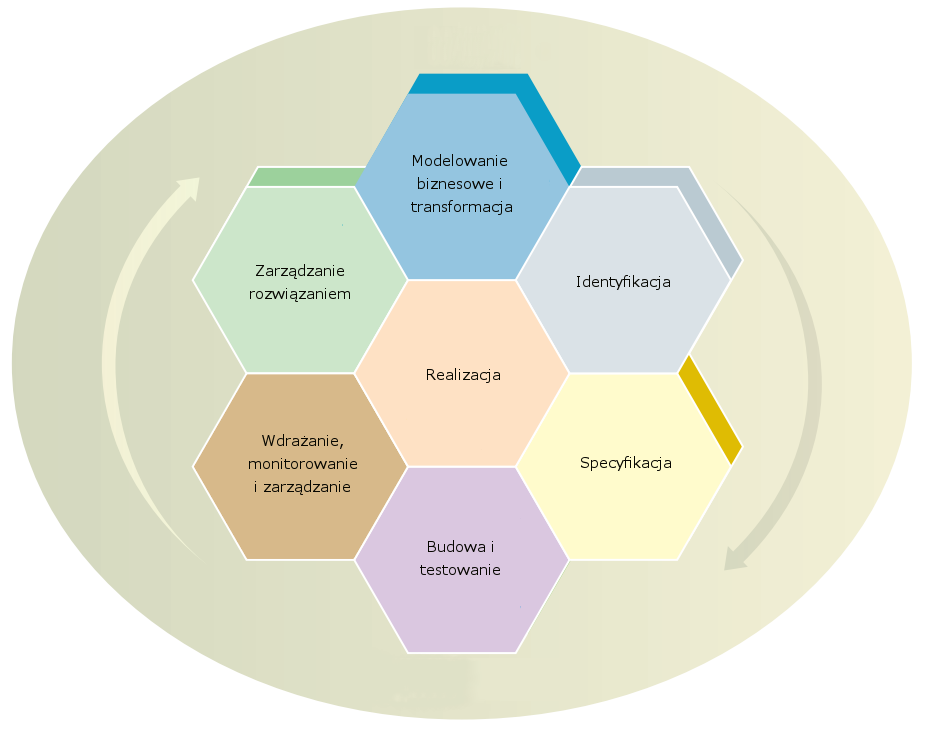
\includegraphics[width=14cm]{img/soma_fractal_lifecycle.png}
\caption[Fraktalne podejście do budowy systemów - fazy metody SOMA.]{Fraktalne podejście do budowy systemów - fazy metody SOMA. \cite{SOMAArsIBMJour}}\label{soma_fractal_lifecycle}
\end{centering}
\end{figure}

Charakterystyczną cechą dla SOMA jest również pojęcie przypadku usługowego (ang. \textit{service case}), który identyfikuje \quotedblbase reużywalny\textquotedblright (ang. \textit{reuse}) zbiór operacji usługi. Ważne jest, aby zidentyfikować taki zestaw usług, który łącznie pozwala na spełnienie celów biznesowych. \cite{PlatIntGor}

W fazie modelowania biznesowego i transformacji funkcjonowanie organizacji jest modelowane, symulowane i optymalizowane. Na tym etapie wyszczególnia się również główny obszar przekształcenia danej jednostki - podstawowy dla kolejnych projektów opierających się na pozostałych fazach SOMA. Modelowanie biznesowe i transformacja jest opcjonalnym elementem metody, ale ściśle zalecanym. 

Realizacje SOA mają hybrydową naturę i z reguły obejmują wiele typów rozwiązań. W fazie zarządzania rozwiązaniem inicjowany jest projekt oraz wybierany odpowiedni scenariusz realizacji. Występuję kilka możliwych scenariuszy: wytwarzania oprogramowania (ang. \textit{custom development}), integracji pakietów aplikacji (ang. \textit{package application integration}). W tym etapie tworzona jest również konfiguracja metody dostosowana do potrzeb danego projektu. Ponadto zdefiniowaniu podlegają: zadania, role, produkty pracy oraz poradniki. \cite{SOMAArsIBMJour}

Faza identyfikacji związana jest z identyfikacją trzech elementarnych dla SOA konstrukcji: usług, komponentów oraz usług. \cite{PlatIntGor} Do zadań tego etapu należy: dekompozycja obszarów biznesowych (Domain Decomposition), modelowanie usług w kontekście celów biznesowych (Goal-Service Modeling) oraz analiza istniejących zasobów IT (Existing Assets Analysis). \cite{SOMAibmRosSuda} Do produktów końcowych tej fazy zalicza się listę kandydujących usług do realizacji oraz powiązań między nimi. \cite{PlatIntGor}

Podczas specyfikacji usług projektowane jest rozwiązanie. Powstaje projekt podstawowy oraz niektóre elementy projektu szczegółowego. Analizowane są zasoby IT pod kątem zależności ze zidentyfikowanymi usługami w poprzedniej fazie, przepływami oraz zdarzeniami. Metoda dostarcza gotowe szablony, wzorce oraz techniki wykorzystywane w celu określenia usług, przepływów i komponentów. 

W skład fazy specyfikacji wchodzą następujące elementy:
\begin{itemize}
\item{Identyfikacja zależności między usługami - w oparciu o szczegółowy przegląd danej usługi możliwe jest odkrycie jej zależności z innymi usługami lub aplikacjami. Mogą okazać się one niezbędne do dostarczenia niektórych funkcjonalności.}
\item{Test papierka lakmusowego (ang. \textit{service litmus test} - powiązany z podejmowaniem decyzji dotyczących ekspozycji.}
\item{Identyfikacja kompozycji usług i przepływów - przegląd procesów biznesowych oraz obszarów funkcjonalnych umożliwia ustalenie kompozycji usług z innych usług i ich przepływów dostarczających pożądaną funkcjonalność biznesową.}
\item{Identyfikacja wymagań niefukncjonalnych - wymagania definiujące oczekiwany poziom usług.}
\item{Definicja specyfikacji komunikatów - obejmuje identyfikację i specyfikację formatu oraz zawartości komunikatów wejściowych i wyjściowych dla usług.}
\item{Dokumentacja decyzji dotyczących zarządzania stanem.}
\end{itemize}

Faza realizacji związana jest ze sprawdzaniem stabilności i realizowalności zaprojektowanego rozwiązania poprzez budowę prototypów. Zadanie to powinno mieć miejsce we wczesnym etapie projektu, aby zminimalizować niepowiedzenia i wyeliminować niepotrzebne ryzyka. Faza ta stanowi pewnego rodzaju formę technicznego studium wykonywalności. Każdy poziom rozwiązania wiąże się również z wybieranym podejściem lub sposobem realizacji prac.

W skład fazy realizacji wchodzą następujące czynności:
\begin{itemize}
\item{iteracyjna alokacja usług do komponentów,}
\item{przypisanie komponentów w warstwach znajdujących się w architekturze aplikacji,}
\item{identyfikacja i oszacowanie ograniczeń technologicznych, które mogą wpływać na realizowalność zadań.}
\end{itemize}

W fazach implementacji i wdrożenia oraz monitorowania i zarządzania są konstruowane, generowane i łączone usługi, komponenty funkcjonalne i techniczne oraz przepływy. Konstruowane są również poszczególne elementy opakowujące oraz odpowiednie mechanizmy dla istniejących komponentów. Wykonywane są również testy: integracyjne, jednostkowe, komponentów, przepływów oraz systemu dla usług. \cite{PlatIntGor, SOMAArsIBMJour}

\subsection{Produkty SOMA}
Stosowanie SOMA przynosi rezultaty między innymi w postaci utworzonych modelów - usług i informacji. 

Model usług zawiera zbiór informacji dotyczących aktualnie zidentyfikowanych usług w organizacji, które będą wykorzystane do realizacji założonych celów biznesowych oraz procesów. W modelu tym znajdują się również dane opisujące kwestie: biznesowe, funkcjonalne, niefunkcjonalne oraz dotyczące technicznej realizacji. Wyszczególnione są również informacje o hierarchii złożoności, ekspozycji, zależności między usługami oraz wymagania związane z poziomem jakości. 

Model informacji odpowiada za kontekst biznesowy. Zawiera elementy takie jak: model koncepcyjny, decyzje dotyczące realizacji oraz relacje i ekspozycję encji.

Oprócz wymienionych modeli metoda SOMA dostarcza również elementy: kontekst biznesowy, definicję procesów, identyfikację procesów, katalog reguł biznesowych oraz listę zdarzeń biznesowych.

\subsection{Zalety i wady SOMA}
Stosowanie metody SOMA może przynosić szereg korzyści. 

Model usług stanowiący końcowy rezultat etapu modelowania pozwala na łatwe i szybkie opracowanie projektu technicznego, implementację nowych usług oraz udostępnienie usług na podstawie już istniejących. 

Ponadto SOMA zakłada wysoki stopień skalowalności systemów tworzonych zgodnie z jej regułami. Zapewnia elastyczność organizacji w związku ze zmianami biznesowymi oraz umożliwia redukcję kosztów wdrażania nowych usług.

Model usług powstały z zastosowania SOMA jest niezależny od platformy. Można wytwarzać go za pomocą wielu dostępnych na rynku narzędzi: \emph{IBM Rational Software Architect}, \emph{Enterprise Architect}, \emph{ARIS} czy \emph{ModelioSoft}.

Do wad SOMA można zaliczyć fakt, że mimo szczegółowego opisu projektu technicznego usług biznesowych nadal elementy dotyczące ich wdrożenia są przedstawiane tylko szczątkowo.

SOMA doskonale wspiera identyfikację usług zgodnie z zasadą \emph{top-down} w modelach procesów biznesowych i innych artefaktach analizy biznesowej. Specyfikacja usług również jest odpowiednio zdefiniowana. Jednakże definicja przejścia pomiędzy tymi dwiema fazami jest niejednoznaczna i często w projektach powstają z tego z tego powodu różne nieścisłości (jak na przykład duplikaty usług) \cite{MicMetZIMM}. 


\section{Metoda Papazoglou}
\subsection{Service-Oriented Design and Development Methodology by Papazoglou}
\emph{Service-Oriented Design and Development by Papazoglou} również stanowi metodę projektowania architektury systemów informatycznych zorientowanych na usługi. Metoda opiera się ponadto na kilku podstawowych założeniach jak poniżej.
\begin{itemize}
\item{Zarządzanie całym cyklem życia usługi włączając: identyfikację, projektowanie, wdrożenie, wykrycie, stosowanie oraz utrzymywanie.}
\item{Na etapie projektowania ustanowienie platformy i modelu programowania uwzględniającego połączenia, wdrażanie i zarządzanie usługami w obrębie określonego środowiska wykonawczego.}
\item{Stosowanie najlepszych praktyk i narzędzie dla rozwiązań architektury, które są powtarzalne, przewidywalne oraz uwzględniają częste zmiany biznesowe.}
\item{Dostarczanie wysokiej jakości wykonywalnych rozwiązań zorientowanych na usługi, które przestrzegają wymagań \emph{Qos} (\emph{Quality of Service})}.
\end{itemize}

Fundamentem dla powyższych założeń jest to, że cele biznesowe i wymagania zawsze powinny prowadzić do niższego poziomu abstrakcji - kolejno: projektowania, implementacji, testowania oraz transformacji procesów biznesowych w kompozytowe aplikacje. W ten sposób wymagania biznesowe mogą 
być śledzone przez cały cykl życia - od celów biznesowych przez projektowanie oprogramowania oraz zasobów kodu, aż do kompozytowych aplikacji.

\subsection{Fazy metody}
Metoda utworzona przez Papazoglou składa się z elementów (rys. \ref{papazoglou_method_phases}) bazujących na innych metodach takich jak: \emph{Rational Unified Process}, \emph{Component-based development} oraz modelowania procesów biznesowych zaproponowanego przez Paula Harmona w 2003 roku \cite{PapaZog}. 

\begin{figure}[h!tbp]
\begin{centering}
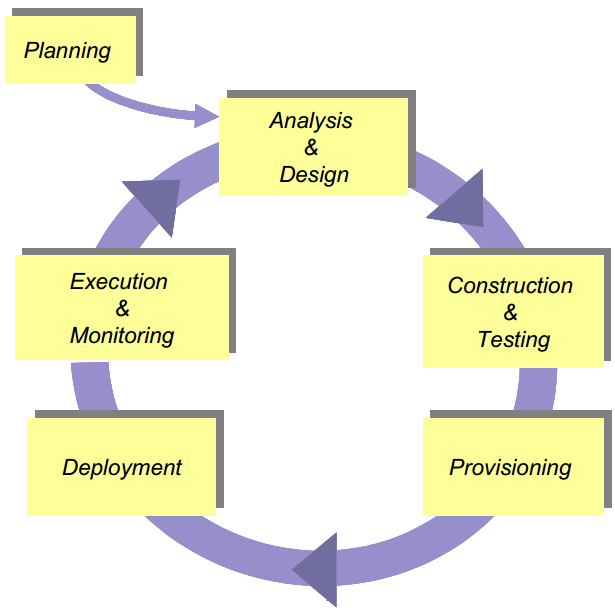
\includegraphics[width=8cm]{img/papazoglou_metoda_fazy.png}
\caption[Fazy metody zaproponowej przez Papazoglou.]{Fazy metody zaproponowej przez Papazoglou. \cite{PapaZog}}\label{papazoglou_method_phases}
\end{centering}
\end{figure} 

Podstawowym celem metody jest jak najlepsza integracja usług oraz osiągnięcie jak najwyższego poziomu ich interoperacyjności. Poszczególne fazy, które wchodzą w składy metody są wymienione poniżej.
\begin{itemize}
\item{Faza planowania (ang. \emph{Planning phase}) - określa prawdopodobieństwo wykonalności, naturę i zakres rozwiązań usługowych w kontekście danej organizacji.  Istotne jest, żeby technologia usługowa pasowała jak najlepiej do obecnego charakteru organizacji. Kluczowe w tej fazie jest dlatego bardzo dobre poznanie obecnego środowiska biznesowego. Czynności związane z fazą planowania obejmują analizę potrzeb biznesowych jako mierzalne cele,  przegląd obecnie wykorzystywanych technologii, ustalenie koncepcji wymagań dotyczących nowego środowiska i mapowanie tych wymagań na nowe lub dostępne implementacje.}

\item{Faza analizy (ang. \emph{Analysis phase}) - w trakcie tej fazy wcześniej zebrane wymagania poddawane są analizie. Postawione uprzednio cele biznesowe podlegają przeglądowi. Analitycy biznesowi tworzą kompletny model procesów typu \emph{as-is} umożliwiając tym samym zapoznanie się z obecnie dostępnymi usługami i procesami biznesowymi. Po udostępnieniu tego modelu organizacja projektuje, symuluje i analizuje potencjalne zmiany do obecnego stanu systemu. Określa również wskaźnik rentowności \emph{ROI} (\emph{Return On Investment}) wynikający ze zmian w panujących procesach biznesowych. Produktem tej fazy jest model procesów biznesowych typu \emph{to-be}, które będą realizowane przez rozwiązania SOA. Przyjmuje się, że w skład fazy wchodzą następujące czynności: identyfikacja procesów (ang. \emph{Process identification}, określanie zakresu procesów (ang. \emph{Process scoping}), analiza luk biznesowych (ang. \emph{Business gap analysis}), analiza realizacji procesów (ang. \emph{Process realization analysis}).}

\item{Faza projektowania (ang. \emph{Design phase}).
Projektowanie systemu zorientowanego usługowo wymaga od projektantów dostarczenia modeli i dobrze zdefiniowanych interfejsów dla wszystkich ważnych komponentów usług. Projektowanie usług bazuje na podejściu wykonywania równolegle dwóch ścieżek: jedna do produkcji usług (ewentualnie z wcześniej utworzonych elementów), natomiast druga związana jest z asemblacją usług reużywalnych (wielokrotnego użytku). Projektowanie usług, podobnie jak analiza usług posiada swoje własne specjalne charakterystki i techniki. Faza projektowania rozpoczyna się od rozważenie kilku istotnych problemów: zarządzania usługami i ziarnistostością komponentów (ang. \emph{Managing Service and Component Granularity}, projektowanie reużywalności usług (ang. \emph{Designing for service reuse}) i ich kompozytowości (ang. \emph{Designing for service composability}).}

\item{Faza specyfikacji usług (ang. \emph{Service specyfing phase}) - składa się z trzech równie istotnych elementów: specyfikacji strukturalnej (ang. \emph{Structural specification}), specyfikacji zachowań (ang. \emph{Behavioural specification}) oraz specyfikacji polityk (ang. \emph{Policy specification}). Podczas tej fazy, interfejsy usług, które zostały wyszczególnione w fazie analizy są definiowane na podstawie kryteriów powiązań (ang. \emph{coupling}) i spójności (ang. \emph{cohesion}).}

\item{Faza specyfikacji procesów biznesowych (ang. \emph{Specifying business processes}) - dzieli się na 3 mniejsze etapy: opisywanie struktury procesów biznesowych (ang. \emph{Designing the business process structure}), opisywanie ról biznesowych (ang. \emph{Describing business roles}) oraz rozważanie zagadnień niefunkcjonalnych związanych z procesami biznesowymi (ang. \emph{Non-functional business process concerns}).}

\item{Faza konstrukcji usług (ang. \emph{Service construction phase}) - obejmuje definicję opisów interfejsów oraz definicję opisów implementacji. Tworzone są usługi typu \emph{Web Service} lub przekształcane istniejące.}

\item{Faza testowania usług (ang. \emph{Testing phase}) - testowanie usługi jest ogólnie scharakteryzowane jako walidacja mająca na celu sprawdzenie, że postawione wymagania zostały spełnione, a osiągnięte rezultaty są na akceptowalnym poziomie (zgodnie z obowiązującymi standardami założonymi w trakcie analizy, projektowania i implementacji).} 

\item{Faza wdrażania usług (ang. \emph{Deployment phase}) - polega na publikacji interfejsu oraz definicji implementacji tej usługi. Jej zasięg obejmuje inne procesy, aplikacje oraz organizacje.}

\item{Faza wykonania. (ang. \emph{Execution phase}) - w jej zakres wchodzi upewnienie się czy wszyscy wyznaczeni uczestnicy są w stanie wykonywać daną usługę. W tej fazie \emph{Web service'y} są już w pełni wdrożone i funkcjonalne. Podczas tego etapu usługobiorca może wynaleźć definicję usługi oraz wywołać wszystkie stowarzyszone z nią operacje.}

\item{Faza monitorowania usług (ang. \emph{Monitoring phase}) - monitorowanie poziomu usług jest zdyscyplinowaną metodologią
ustalenia dopuszczalnych poziomów usług, które dotyczą celów biznesowych, procesów i kosztów. W fazie tej następuje wykonanie pomiarów, monitorowanie, raportowanie i poprawianie jakości usług i aplikacji dostarczanych przez rozwiązania zorientowane usługowo. \cite{PapaZog}}
\end{itemize}

\subsection{Zalety i wady metody Papazoglou}
Do zalet metody Papazoglou można zaliczyć przede wszystkim pokrywanie pełnego cyklu wytwarzania usług (ang. \emph{lifecycle coverage}). Metoda Papazoglou doskonale wspiera rozwijanie usług już istniejących dzięki opieraniu fazy analizy na strategii \emph{meet in the middle} oraz swojemu przyrostowemu charakterowi. 

Metoda jest jednakże ciągle w fazie rozwoju i testów. Nie była wdrażana produkcyjnie. \cite{RamErvSOA}


\section{Metoda Thomasa Erl'a}
TODO: A Comparison of SOA Methodologies Analysis And Design Phases 

\subsection{Opis metody}
Metoda Thomasa Erl'a stanowi pierwszą metodologię SOA, która w pełni zasługiwała na komercyjne stosowanie. Stanowi przewodnik jak krok po kroku przejść dwie podstawowe fazy - analizy i projektowania. Opiera się na metodzie \emph{top-down}.

Analiza zorientowana usługowo według Thomasa Erl'a powinna być rozważana w trzech etapach: definicji wymagań biznesowych (ang. \emph{define business requirements}), identyfikacji w istniejących systemach elementów możliwych do automatyzacji (ang. \emph{identify  existing 
automation systems})oraz przygotowania modelu usług kandydujących (ang. \emph{model candidate services}). 

W pierwszej fazie analizy rozpatrywane są cele i zadania organizacji oraz rozważane potencjalne zmiany do obecnych aplikacji (sprawdzane są możliwości ich przekształcenia niezbędne do budowy systemu w oparciu o SOA). Analitycy biznesowi przygotowują model procesów biznesowych \emph{as-is} przeznaczony do wglądu przez wszystkie podmioty biorące udział w wytwarzaniu usługi. 

W kolejnym etapie identyfikowane są elementy procesów organizacji, które mogą zostać poddane automatyzacji. Rozpatrywany jest również utworzony wcześniej model \emph{as-is} pod kątem utworzenia nowych lub modyfikacji istniejących procesów biznesowych. Efektem tego etapu jest przygotowanie modelu procesów biznesowych \emph{to-be}, który będzie implementowany.

Ostatnią fazę analizy stanowi podproces modelowania usług, w którym są identyfikowani oraz uwzględniani na modelach \quotedblbase usług kandydujących\textquotedblright (ang. \emph{service candidates}). \cite{CompSOAMet}

Utworzone modele \quotedblbase usług kandydujących\textquotedblright są wykorzystywane w następnym etapie - projektu zorientowanego usługowo (ang. \emph{Service oriented design}). \quotedblbase Usługi kandydujące\textquotedblright są wówczas szczegółowo specyfikowane i później realizowane jak \emph{Web service'y}.


\subsection{Zalety i wady}
Metoda projektowania SOA zaproponowana przez Thomasa Erl'a może być używana jedynie w połączeniu z innymi metodami. Dostarcza opisy dotyczące zorientowanych usługowo faz analizy i projektu, ale nie precyzuje tak istotnych elementów jak rozpoczęcie projektu SOA oraz jak przeprowadzić analizę biznesową organizacji. Ponadto metoda Thomasa Erl'a nie specyfikuje wystarczająco wykorzystania elementów obecnego systemu. Ponadto role podmiotów biorących udział w działaniu systemu nie są spójnie określone.

Do pozytywnych cech metody można zaliczyć fakt, że wspiera najpopularniejsze standardy i technologie takie jak: BPM, WSDL, WS-BPEL oraz WS-*. Metoda jest również łatwa do zaadaptowania ze względu na dość prosty algorytm stosowania. Metoda Thomasa Erl'a opiera się również na manifeście Agile, który wspiera \quotedblbase zwinne tworzenie oprogramowania\textquotedblright. \cite{OffCompSOAM, RamErvSOA}

\chapter{Opracowanie metody projektowania systemów informatycznych o architekturze SOA}
\section{Wstęp}
W poprzednim rozdziale został dokonany przegląd istniejących metod projektowania systemów informatycznych o architekturze SOA.

Stopień złożoności biznesowej niektórych organizacji jest naprawdę wysoki. Bez zastosowania odpowiedniej, usystematyzowanej metody utworzenie sprawnie funkcjonującego systemu informatycznego stanowi istotny problem. Występuje wiele metod o różnej charakterystyce jednakże niemal każda wykazuje pewne niedociągnięcia.

Większość metod łączy opis sposobu przejścia od stanu początkowego (wyniknięcie potrzeby posiadania systemu informatycznego) do końcowego (utworzenie systemu informatycznego zgodnego z wymaganiami zebranymi w trakcie analizy).  Każda z nich stanowi hierarchicznie uporządkowany zbiór elementów takich jak: fazy, aktywności, zadania oraz kroki. Opierają się również na wykorzystywaniu różnorodnych technik oraz zalecanych języków modelowania i notacji \cite{OffCompSOAM}.

W rozdziale tym zostanie podjęta próba zdefiniowania nowej metody projektowania systemów informatycznych o architekturze SOA oraz porównanie jej charakterystyki z obecnie dostępnymi.


\section{Metoda MatSOA}
MatSOA stanowi autorską metodę projektowania architektury korporacyjnej. Obecne metody posiadają zarówno wiele wad jak i zalet. Różnią się podziałami na etapy, wykorzystywanymi technologiami oraz zakresem stosowalności. MatSOA stanowi połączenie najlepszych cech z już istniejących wzorców. Wprowadza także pewne własne elementy usprawniające projektowanie architektury korporacyjnej. 

MatSOA w odróżnieniu od wielu występujących metod uwzględnia również analizę obecnych systemów (ang. \emph{legacy systems}). Cechę charakterystyczną dla MatSOA stanowi fakt, że do specyfikacji usług wykorzystuje język SoaML stanowiący rozszerzenie dla UML. 

W celu dokładnego opisania metody zostaną przedstawione jej poszczególne fazy oraz związane z nią notacje modelowania. Będą opisane również możliwe narzędzia, które wspierają proces projektowania w oparciu o MatSOA.

Metoda MatSOA składa się z sześciu głównych faz, których sekwencja została przedstawiona na rys. \ref{soam_lifecycle}. Wszystkie fazy zawierają szereg aktywności, z których każda ma przypisaną rolę wykonania oraz określone artefakty wejściowe i wyjściowe.

Faza analizy organizacji oraz wykrywania usług ma równoległy przebieg do analizy obecnych systemów. Produkty wyjściowe powstałe w wyniku dwóch podejść analizy - \emph{top-down} oraz \emph{bottom-up} - są następnie konsolidowane. W kolejnym etapie projektowane są usługi, które z kolei są wykorzystywane do przygotowania procesów biznesowych.

\begin{figure}[h!tbp]
\begin{centering}
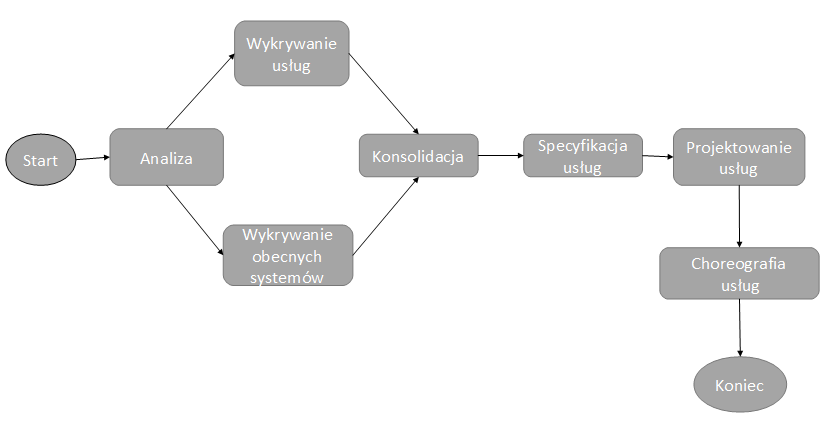
\includegraphics[width=15cm, height=9cm]{img/MetMatSOA_v2.png}
\caption[Fazy metody MatSOA.]{Fazy metody MatSOA.}\label{soam_lifecycle}
\end{centering}
\end{figure}


W tej sekcji pracy zostaną omówione poszczególne fazy metody MatSOA.

\subsection{Analiza}
W celu identyfikacji wymagań organizacji należy rozpatrzyć poszczególne aspekty z nią związane: strategie biznesowe, procesy biznesowe oraz domeny funkcjonalne. W wypadku MatSOA analiza organizacji ma przebieg kilku etapowy oraz powinna być przeprowadzana przez analityka biznesowego.

\subsection*{BMM - Motywacyjny Model Biznesowy}
W pierwszym kroku analizy organizacji w przypadku metody MatSOA tworzony jest motywacyjny model biznesowy (BMM - \emph{Business Motivation Model}). Stanowi on część opisu organizacji. Umożliwia między innymi uchwycenie i przedstawienie w prosty sposób planów biznesowych. Do podstawowych celów BMM zalicza się ponadto:
\begin{itemize}
\item{identyfikację czynników, które powodują konieczność utworzenia planu,}
\item{identyfikację oraz definicję elementów niezbędnych do wykorzystania w układanym planie,}
\item{określenie, jak wymienione elementy są ze sobą powiązane.}
\end{itemize}

BMM został stworzony przez BRG (\emph{Business Rules Group}), a następnie w 2005 roku grupa OMG jako pierwsza poddała BMM formalnej specyfikacji. Utworzyła również schemat, na którym można opierać się przy tworzeniu BMM (rys. \ref{BMM_schem}) \cite{AnaWesHal}.

\begin{figure}[h!tbp]
\begin{centering}
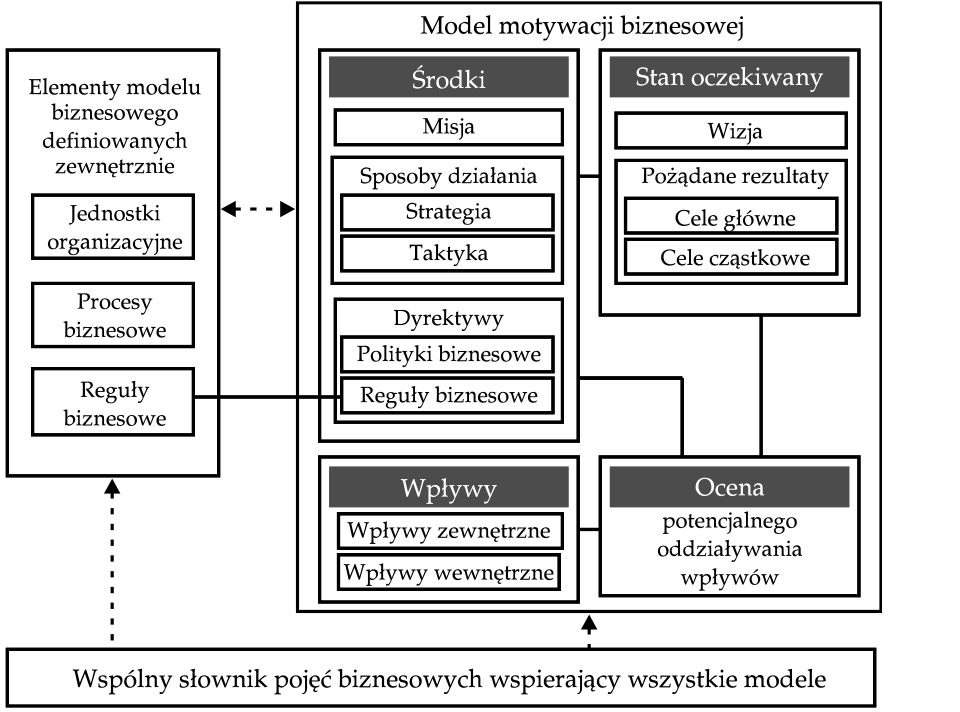
\includegraphics[width=12cm, height=11cm]{img/BMM_PL.png}
\caption[Schemat ogólny BMM utworzony przez organizację OMG.]{Schemat ogólny BMM utworzony przez organizację OMG. \cite{BMMOmg}}\label{BMM_schem}
\end{centering}
\end{figure}

Motywacyjny model biznesu stanowi element integrujący względem innych modeli (np. modeli procesów biznesowych, modeli reguł biznesowych) i nie jest uwarunkowany (zależny) metodycznie od innych standardów. BMM stanowi pewnego rodzaju ramę koncepcyjną pozwalającą stworzyć repozytorium modeli wspólnie odwzorowujących model biznesowy danej organizacji. W BMM istotną rolę odgrywa wspólny słownik pojęć biznesowych zapewniający spójność semantyczną tworzonych modeli.

Do podstawowych elementów BMM zalicza się: stan oczekiwany (ang. \emph{Ends}) - coś co dana organizacja chce osiągnąć, wizję (ang. \emph{Vision}) - ogólne przedstawienie pożądanych osiągnięć, cele (ang. \emph{Goals}) - wynikają z utworzonej wcześniej wizji, zadania (ang. \emph{Objectives}) - wynikają z celów postawionych przez organizację, misję (ang. \emph{Mission}), strategie (ang. \emph{Strategies}) i taktyki (ang. \emph{Tactics}) \cite{AnaWesHal}. 

W kolejnej fazie analizy organizacji na podstawie BMM są identyfikowane procesy biznesowe niezbędne do wspierania jej strategii działania. Ustalane są również kryteria (np. częstość zmian w procesach, obecny poziom możliwej integracji z istniejącymi systemami oraz stopień, w którym procesy mogą być z góry określane i wydzielane) na podstawie, których wyszczególniany jest inny typ lub części procesów biznesowych, które powinny być wspierane przez systemy SOA.

Procesy biznesowe definiuje się jako ustrukturyzowany i zmierzony ciąg czynności, który jest zaprojektowany do osiągnięcia określonego wyniku\cite{PlatIntGor}. Każda z czynności poddawana jest klasyfikacji zgodnie z tym czy może być wykonywana automatycznie (\emph{Business service}), czy wymaga interakcji między użytkownikiem, a systemem (\emph{User interaction}) oraz czy jej działanie ma charakter wyłącznie ręczny (\emph{Manual}).

MatSOA zakłada identyfikowanie mierzalnych, udokumentowanych i powtarzalnych procesów. Modele procesów biznesowych powinny być budowane na różnych poziomach szczegółowości i mieć budowę hierarchiczną. Modele wysokiego poziomu powinny określać przepływ pomiędzy poszczególnymi podmiotami (rolami), a w dalszej kolejności być dekomponowane na procesy, w których wykonawcami są pojedyncze osoby. 

Zalecaną notację modelowania stanowi BPMN (\emph{Business Process Modelling Notation}). Określenie przepływu danych w procesie nie jest wymagane na tym etapie. Wykonywanie uproszczonych modeli procesów biznesowych, w których uwzględnione są jedynie aktywności ma na celu przede wszystkim utworzenie zarysu jak będzie wyglądała integracja z poszczególnymi systemami.

Równolegle do modelowania procesów biznesowych powstaje warstwowy model domen funkcjonalnych (ang. \emph{FD - Functional Domains}). Proponowaną notacją dla FD są diagramy przypadków użycia UML. Każda aktywność modelu procesu biznesowego jest przypisywana do domeny funkcjonalnej. Modelowanie procesów biznesowych i FD powinno być wykonywane iteracyjnie. Połączenia aktywności procesów i domen funkcjonalnych pomaga później w zapewnieniu reużywalności usług.

\subsection*{Wymagania funkcjonalne}
Po zidentyfikowaniu wymagań od klienta należy przeprowadzić ich analizę. Wykryte wymagania są na tym etapie uszczegóławiane oraz określane są ich priorytety oraz ryzyka. Odrzucane są również wymagania sprzeczne lub nieprawidłowe.

Analiza wymagań funkcjonalnych pozwala na zidentyfikowanie i opisanie pożądanego zachowania systemu. W przypadku rozbudowy systemów identyfikowane są nowe funkcjonalności, o które system ma zostać rozszerzony.

Analiza wymagań funkcjonalnych przedstawiana jest za pomocą diagramów przypadków użycia.

\subsection*{Wymagania niefunkcjonalne}
W metodzie MatSOA na wymagania niefunkcjonalne składa się opis atrybutów jakościowych jakim ma podlegać tworzony system, model domeny oraz wykrywanie dotychczasowych systemów. Zdarza się, że w niektórych metodach do wymagań niefunkcjonalnych zaliczana jest także analiza dotychczasowych systemów. W MatSOA ten etap jest zawarty w późniejszej fazie. 

Model domeny przedstawia podmioty wchodzące w skład, w której działa dana organizacja lub przedsiębiorstwo. Przedstawia również relacje pomiędzy danymi podmiotami. Modelowana jest za pomocą diagramu przypadków użycia UML.

Wykrywanie obecnych systemów jest bardzo ważnym etapem analizy. Należy określić, które z systemów dotychczas występujących w organizacji będą zależne od wprowadzanych nowych funkcjonalności.

Do atrybutów jakościowych w przypadku MatSOA zalicza się przede wszystkim spełnianie podstawowych pryncypiów SOA. Są to przede wszystkim: luźne powiązania, autonomiczność, enkapsulacja oraz reużywalność usług.

\subsection{Identyfikacja usług}
Identyfikacja usług stanowi kolejny etap metody MatSOA. W jej efekcie otrzymywany jest model kandydatów usług wykorzystywany w kolejnych fazach metody. 
Faza ta powinna się rozpoczynać od wykrycia kandydatów usług (ang. \emph{Service Candidates}). 

Owi kandydaci usług stanowią pewnego rodzaju propozycje dotyczące usług.  W późniejszym etapie poddawane są specyfikacji pod warunkiem, że odpowiednia usługa nie występuje w dotychczasowym systemie.

Modele kandydatów usług są tworzone na podstawie wcześniej ustalonych wymagań funkcjonalnych w sposób zorientowany na usługi. Artefakty modelowane w fazie analizy wymagań są odpowiednio transformowane do kandydatów usług. Stanowi to wstępny etap do przygotowania modeli docelowych usług (rys. \ref{MatSOAServicesIdent}). 

\begin{figure}[h!tbp]
\begin{centering}
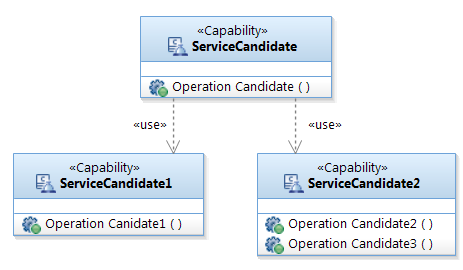
\includegraphics[width=10cm, height=6cm]{img/service_candidates.png}
\caption[Identyfikacja usług - metoda MatSOA.]{Identyfikacja usług - metoda MatSOA.}\label{MatSOAServicesIdent}
\end{centering}
\end{figure}

Do modelowania kandydatów usług wykorzystywany jest element języka SoaML - Capability. Każdy element Capability zawiera operacje oraz można wykazywać zależności pomiędzy nimi za pomocą Usage Dependency. W tabeli (\ref{tabela_service_candidates_soaml}) zostały zawarte mapowania kandydatów usług na poszczególne elementy języka SoaML.

\begin{table}[!htbp]
\begin{center}
\begin{small}
\begin{supertabular}{|p{6cm}|p{7cm}|}\hline
\textbf{Element kandydata usługi} & \textbf{Element w języku SoaML}\\\hline
Kandydat usługi &	Capability (klasa UML ze stereotypem  \quotedblbase Capability\textquotedblright)  \\\hline
Operacja kandydata usługi &	Operacja wewnątrz elementu Capability \\\hline
Zależność kandydata usługi &	Usage Dependency - zależność pomiędzy poszczególnymi Capability \\\hline
\end{supertabular}
\end{small}
\end{center}
 \caption{Mapowanie kandydatów usług na elementy języka SoaML.}
 \label{tabela_service_candidates_soaml}
\end{table}

Wykrywanie usług może mieć iteracyjny charakter. Już na tym etapie powinno się uwzględniać wymagania niefunkcjonalne związane z atrybutami jakościowymi. Należy przejrzeć czy wykryte operacje nie są wewnętrzne. Musimy również rozważyć szanse na reużywalność poszczególnych kandydatów usług. 


\subsection*{Analiza obecnych systemów i zasobów}
Analiza istniejących systemów (ang. \emph{Legacy systems}) oraz zasobów stanowi bardzo istotny etap metody MatSOA. Wykonywyana jest równolegle do wykrywania nowych usług. Umiejętne przeprowadzenie tej fazy często może znacznie zredukować koszty wprowadzania nowych funkcjonalności w systemach organizacji. Na tym etapie identyfikowane są elementy takie jak: istniejące aplikacje, standardy branżowe, modele oraz pozostałe zasoby niezbędne do realizacji usług. 

W założeniu metody MatSOA analityk systemowy powinien zidentyfikować istotne systemy. Następnie te rozpoznane systemy są analizowane pod kątem przydatnych funkcjonalności. Często się zdarza, że nie wszystkie elementy dotychczasowych systemów mogą być wykorzystane bezpośrednio. Jeśli jest to usługa SOA wprowadza się wówczas odpowiednie modyfikacje do obecnych systemów. W innych wypadkach należy rozważyć czy jest szansa wykorzystania ich poprzez opakowującą je usługę (ang. \emph{wrapper}). Sposobów na używanie istniejących zasobów jest wiele: API, dostępne bazy danych, komponenty oprogramowania, które mogą być opakowane oraz wywołanie komendy z wiersza poleceń.

Takie opakowane elementy są następnie modelowane jako kandydaci usług wraz z odpowiadającymi im operacjami. Istotne jest, żeby analityk wybierał tylko te usługi, które są powiązane z ustalonymi wymaganiami funkcjonalnymi.

Podobnie jak w przypadku etapu identyfikacji usług analizę obecnych systemów i zasobów można wykonywać w sposób iteracyjny. W każdym kroku powinno następować sprawdzanie czy utworzony model kandydatów usług spełnia wymagania niefunkcjonalne. Jeśli wykryte usługi naruszają istotnie takie zasady SOA jak \quotedblbase luźne powiązania\textquotedblright bądź \quotedblbase reużywalność\textquotedblright to wtedy rozważana jest ich modyfikacja.

\subsection{Konsolidacja}
Po wykryciu nowych usług metodą typu \emph{top-down} i identyfikacji usług istniejących systemów typu \emph{bottom-up} konieczna jest ich odpowiednia konsolidacja. Faza ta wykonywana jest przez architekta systemowego i może mieć charakter iteracyjny.

Operacje wywodzące się z systemów już istniejących mają pierwszeństwo. Istotne jest dlatego tutaj rozważenie czy operacje w wykrytych poszczególnych kandydatach usług na podstawie analizy wymagań funkcjonalnych nie występują w dotychczasowych systemach. W trakcie konsolidacji ponownie należy wziąć pod uwagę wymagania niefunkcjonalne i jeśli wyniknie konieczność wykonać odpowiednie modyfikacje w systemie dotychczasowym. Zmiana w obecnym systemie może zostać jedynie rozważona jeśli rozbieżność pomiędzy wymaganiami i aktualnym systemem jest zbyt duża. 

W wyniku konsolidacji tworzony jest model kandydatów usług uwzględniający rozszerzenie dotychczasowych elementów systemu o nowe funkcjonalności.

\subsection{Specyfikacja usług}
Po ustaleniu modeli kandydatów usług poszczególne usługi są specyfikowane. Określane są parametry wejściowe i wyjściowe oraz opisywane poszczególne kontrakty usługowe. Na tym etapie tworzony jest również model danych. Przebieg wywołań pomiędzy poszczególnymi interfejsami usług opisywany jest za pomocą diagramu sekwencji (każdy interfejs usługi przedstawiany zostaje jako osobny lifeline).

W efekcie specyfikacji usług tworzone są modele jak na rys. \ref{}

//TODO: Dodać model przykładowej specyfikacji usług

\subsection{Projektowanie usług}
Po ustaleniu modelu operacji usług, poszczególne usługi mogą zostać zaprojektowane. Celem tej fazy jest na podstawie utworzonej wcześniej specyfikacji usług przygotowanie odpowiednich komponentów usług (ang. \emph{Service Components}). 

Do realizacji tych celów zostaną wykorzystane odpowiednie elementy języka SoaML (tab. \ref{tabela_service_projects_soaml}). Istotnym elemenetem są uczestnicy usługi (Participant).  Na podstawie wcześniej utworzonych modeli należy zdecydować, którzy uczestnicy będą wykorzystani i jak zostaną przyłączeni do funkcjonującego systemu. Element Participant zostanie wykorzystany do przedstawienia modelu komponentu, który będzie dostarczał (element Service) lub konsumował (element Request) poszczególne usługi. 

Utworzone komponenty można łatwo integrować z pozostałymi częściami systemu. 

\begin{table}[!htbp]
\begin{center}
\begin{small}
\begin{supertabular}{|p{6cm}|p{7cm}|}\hline
\textbf{Element projektu usługi} & \textbf{Element w języku SoaML}\\\hline
Interfejs usługi (ang. \emph{Service interface}) &	ServiceInterface - klasa UML ze stereotypem  ServiceInterface  \\\hline
Dostarczana operacja (ang. \emph{Provided operaton}) &	Operacja wewnątrz interfejsu realizowana przez element ServiceInterface \\\hline
Realizowana operacja (ang. \emph{Realized operation}) &	Operacja, która jest połączona z elementem ServiceInterface poprzez użycie Usage Dependency z UML \\\hline
Komponent usługi (ang. \emph{Service component}) &	Usage Dependency - Uczestnik - komponent UML nazywany Participant \\\hline
Dostarczana usługa (ang. \emph{Provided service}) &	Usługa - port UML ze stereotypem Service  \\\hline
Wymagana usługa (ang. \emph{Required service}) &	Zapytanie - port UML ze stereotypem Request \\\hline
Wewnętrzne zachowanie (ang. \emph{Internal behaviour}) &	Aktywność UML, która jest dodawana jako OwnedBehaviour do elementu Participant \\\hline
Port &	Element Port wykorzystywany przy tworzeniu dostarczanej usługi\\\hline
Kanał usług &	Element ServiceChannel wykorzystywany przy tworzeniu połączeń pomiędzy konsumentami i producentami usług\\\hline
\end{supertabular}
\end{small}
\end{center}
 \caption{Projektowanie usług w odwzorowaniu na poszczególne elementy języka SoaML.}
 \label{tabela_service_projects_soaml}
\end{table}

\subsection{Choreografia usług}
Choreografia usług stanowi końcową fazę metody MatSOA. Tworzone są moduły SCA (ang. \emph{Service Component Architecture}), w których opisywany jest sposób komunikacji w systemie między komponentami. Poszczególne wywołania usług poddawane są choreografii z wykorzystaniem WS-BPEL. Wywołania usług definiowane są jako aktywności, a w przypadku wystąpienia błędów wyrzucane są odpowiednie wyjątki. Jeśli zachodzi potrzeba transformacji komunikatów do wymaganej formy przez producenta lub konsumenta można utworzyć odpowiednie mediacje. Przed wywołaniem usługi komunikat zostaje przetworzony wówczas do akceptowalnej formy.

Przygotowane moduły SCA są wdrażane bezpośrednio na serwer gdzie definiowane są połączenia punktów końcowych do poszczególnych usług zewnętrznych.

\subsection{Końcowy produkt}
Celem zastosowania metody MatSOA jest doprowadzenie do utworzenia systemu informatycznego opierającego swoje działanie na kooperacji usług. System utworzony zgodnie z paradygmatami MatSOA powinien charakteryzować się dużą ziarnistością i wysokim poziomem skalowalności.

Istotne jest, aby w trakcie identyfikacji oraz specyfikacji usług konfrontować modele z wymaganiami niefunkcjonalnymi z wyszczególnionymi atrybutami jakościowymi.

\chapter{Weryfikacja koncepcji na przykładzie systemu bankowego}
\section{Wstęp}
Systemy bankowe często charakteryzują się dużą złożonością i panuje w nich wiele różnorodnych procesów biznesowych. Odpowiednio zaprojektowany system jest więc niezbędny we współczesnej bankowości.
 
W niniejszym rozdziale metoda MatSOA zostanie poddana weryfikacji pod względem przydatności do tworzenia tego typu systemów. Systemy bankowe to dziedzina bardzo szeroka dlatego zostanie przedstawiony projekt tylko niewielkiej części wyobrażonego systemu. Niemniej jednak na tym przykładzie zostaną zaprezentowane wszystkie fazy autorskiej metody.

W oparciu o zasady \emph{Model Driven Development (MDD)} zostanie również przedstawiony proces implementacji zgodnie z utworzonymi modelami. Wdrożenie systemu wymaga również istotnych rozważeń związanych z konfiguracjami środowiska, na którym będzie funkcjonować. Zostaną więc też przedstawione szczegóły techniczne dotyczące budowania systemu oraz jego instalacji na serwerach.

Na zakończenie rozdziału zostaną opisane również testy jakim zostanie poddany system po utworzeniu.

\section{Projektowanie systemu bankowego w oparciu o utworzoną koncepcję}
Przykład wykorzystany w pracy będzie oparty na wymyślonej przez autora koncepcji organizacji. Zostaną przedstawione i poddane rozważaniom jednakże tylko wybrane modele mające na celu jak najlepszą prezentację poszczególnych faz metody MatSOA.

Modele w rozdziale zostały przygotowane z wykorzystaniem narzędzi Rational Software Architect w wersji 8.5 wraz z doinstalowanym dodatkiem do obsługi języka SoaML oraz WebSphere Integration Developer w wersji 7.0, w którym zdefiniowane połączenia pomiędzy komponentami i zaimplenetowano całość systemu.

\subsection{Opis sytuacji biznesowej}
FrostRes stanowi niewielki bank krajowy. Ze względu na krótki pobyt na rynku pełni tylko podstawową liczbę usług związanych przede wszystkim z utrzymywaniem kont klientów i wykonywaniem podstawowych operacji finansowych. 
 
Bank posiada obecnie system informatyczny, jednakże nie jest on wystarczający na znaczną ilość klientów, która stale się zwiększa. Wymaga także modernizacji związanej z wprowadzonymi ustawami rządowymi.  

W obecnej chwili system umożliwia zarządzanie kontami klientów (otwarcie i zamknięcie konta, pobranie informacji o koncie, pobranie historii operacji wykonywanych na koncie) oraz obsługę transakcji finansowych (przelewy krajowe oraz wpłata i wypłata pieniędzy). 

Zarząd banku prognozuje wykonanie szeregu zmian w istniejącym systemie. Ze względu na fakt, że organizacja dopiero się rozwija i ma ograniczony budżet zdecydowano się jak na razie na wprowadzenie tylko jednej nowej usługi - przelewów międzynarodowych. Podstawowe wymaganie stanowi fakt, żeby kraje uczestniczące w transakcjach przelewów posiadały rachunki walutowe spełniające normy IBAN (International Bank Account Number). Oprócz tego ustalono, że system po modernizacji ma być w pełni zgodny z pryncypiami SOA. 

Inna istotna zmiana związana jest z nową ustawą wprowadzoną przez rząd, która wprowadziła konieczność weryfikacji każdego przelewu powyżej 10000 złotych przez usługę udostępnioną przez Narodowy Bank Polski. W związku z tym konieczna będzie integracja z usługą weryfikacji przelewów ze strony Narodowego Banku Polskiego. W systemie wykorzystywane są dane o wysokim stopniu poufności dlatego wszelkie integracje z systemami zewnętrznymi muszą ścisło podlegać standardom bezpieczeństwa wymiany komunikatów w architekturze usługowej.

Ze względu na fakt, że w przyszłości planowane są kolejne modernizacje oraz rozszerzenia, system musi wykazywać się stosunkowo dużą skalowalnością. Istotne jest również, żeby stworzony system charakteryzował się wysokim poziomem ziarnistości oraz zapewniał jak największą reużywalność usług. 


\subsection{Analiza}
Analizy zostanie przedstawiona w podziale na poszczególne etapy zgodne z metodą MatSOA. Rozpocznie się od opisania BMM, na podstawie którego zostanie utworzony uproszczony model procesu biznesowego. W kolejnych krokach zostaną przedstawione rozważania dotyczące wymagań funkcjonalnych i niefunkcjonalnych.

\subsection*{Przygotowanie Business Motivation Model (BMM)}
Budowa systemu dla FrostRes została rozpoczęta od przygotowania motywacyjnego modelu biznesu. Tworzenie BMM jest krokiem opcjonalnym metody MatSOA jednakże stanowi bardzo dobry wstęp dla analizy. W zależności od stopnia złożoności sytuacji biznesowej może wykazywać się różnym poziomem szczegółowości. Modernizacja banku FrostRes nie stanowi zbyt złożonego problemu biznesowego, dlatego tworzony BMM będzie zawierał tylko najbardziej podstawowe elementy.

Przygotowanie BMM przedstawionego na rys. \ref{BMM_frostres} rozpoczęto od rozważenia środków (element \emph{<<Means>>}). Następnie określono misję (element \emph{<<Mission>>}), ustalono strategie (elementy \emph{<<Strategy>>}) oraz ułożono odpowiednie taktyki (elementy \emph{<<Tactic>>}) wdrażania biznesu. Na podstawie analizy powyższych elementów wyodrębniono proces biznesowy, który będzie realizował \quotedblbase Obsługę przelewu międzynarodowego\textquotedblright (element \emph{<<Business Process>>}). 

W BMM opisano również stan oczekiwany (element \emph{<<End>>}) przez bank FrostRes. Dekompozycję rozpoczęto tym razem od określenia wizji (element \emph{<<Vision>>}) powiązanej bezpośrednio z utworzonym wcześniej opisem misji. Następnie przedstawiono cele główne (element \emph{<<goal>>}) oraz cząstkowe (element \emph{<<Objective>>}).

\begin{figure}[h!tbp]
\begin{centering}
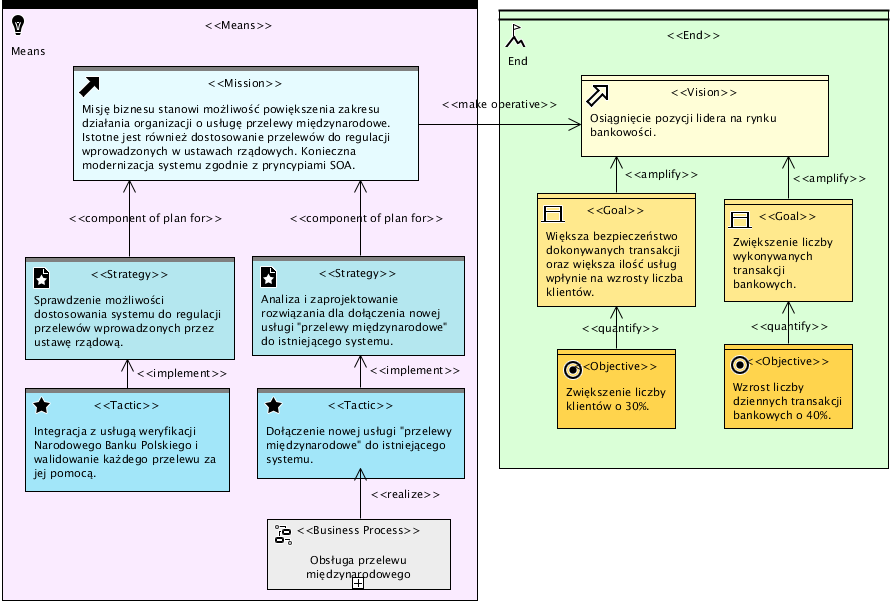
\includegraphics[width=16cm, height=12cm]{img/bmm_model_frostres.png}
\caption[Model BMM dla modernizacji banku FrostRes]{Model BMM dla modernizacji banku FrostRes.}\label{BMM_frostres}
\end{centering}
\end{figure}

W następnym kroku wykryty wcześniej proces \emph{Obsługa przelewu międzynarodowego} (rys. \ref{proces_operacja_przeleu_miedzynarodowego}) opisano z wykorzystaniem języka BPMN. Opiera się na usługach poddanych pewnego rodzaju \emph{choreografii}. Ma on charakter jedynie poglądowy. Na tym etapie nie jest zdefiniowany jeszcze przepływ danych pomiędzy poszczególnymi aktywnościami procesu. Tworzenie uproszczonej formy modelu procesu w początkowej fazie cyklu życia projektu SOA ma na celu jak najwcześniejsze wykrycie istotnych problemów związanych z logiką przebiegu wywoływania usług pomiędzy poszczególnymi podmiotami. Pozwala to także na ewentualne dostosowanie uczestnikom integracji wystawianych interfejsów. Poniżej został opisany przebieg procesu wraz z przepływem pomiędzy uczestniczącymi rolami.

//TODO: Zaaktualizować model procesu
\begin{figure}[h!tbp]
\begin{centering}
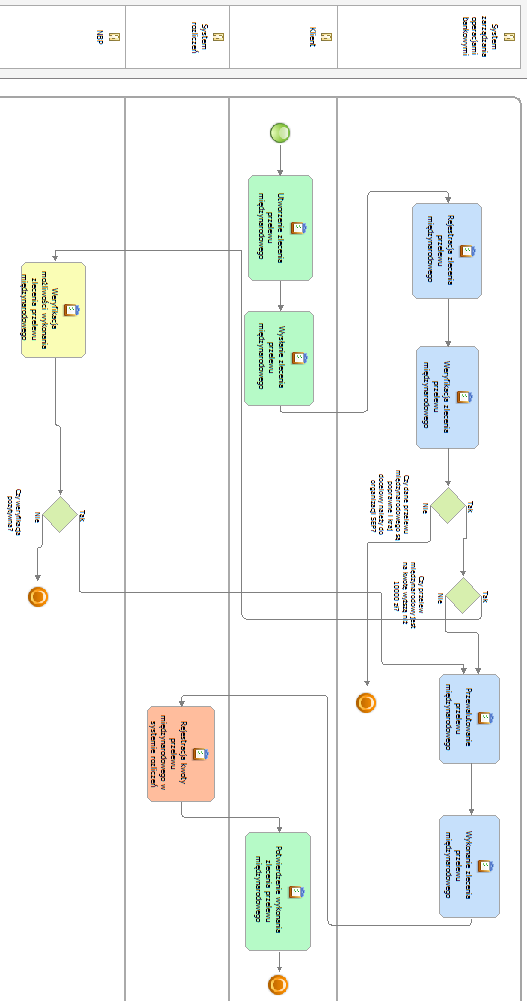
\includegraphics[width=12.5cm,height=20cm]{img/proces_operacja_przeleu_miedzynarodowego.png}
\caption[Proces obsługi przelewu międzynarodowego - diagram BPMN.]{Proces obsługi przelewu międzynarodowego - diagram BPMN.}\label{proces_operacja_przeleu_miedzynarodowego}
\end{centering}
\end{figure}

//TODO: zaaktualizować scenariusz
\begin{flushleft}
1. Klient tworzy zlecenie przelewu międzynarodowego.\\
2. Klient wysyła zlecenie przelewu międzynarodowego.\\
3. SZOB rejestruje zlecenie przelewu międzynarodowego.\\
4. SZOB weryfikuje zlecenie przelewu międzynarodowego.\\
\textit{{[}dane przelewu są poprawne; przelew międzynarodowy na kwotę wyższą niż 10000 złotych{]}}\\
\hspace{1ex}5.1 NBP weryfikuje możliwość wykonania przelewu.\\
\hspace{1ex}{[}pozytywna weryfikacja przelewu{]}\\
\hspace{2ex}6.1.1 SZOB przewalutowuje przelew międzynarodowy.\\
\hspace{2ex}7.1.1 SZOB wykonuje zlecenie przelewu międzynarodowego.\\
\hspace{2ex}8.1.1 SR rejestruje kwotę przelewu międzynarodowego w systemie rozliczeń.\\
\hspace{2ex}9.1.1 System wyświetla potwierdzenie wykonania przelewu klientowi.\\
\hspace{2ex}\textit{{[}dane przelewu są poprawne; przelew na kwotę niższą niż 10000 złotych{]}}\\
\hspace{1ex}5.2. SZOB przewalutowuje przelew międzynarodowy.\\
\hspace{1ex}6.2. SZOB wykonuje zlecenie przelewu międzynarodowego.\\
\hspace{1ex}7.2. SR rejestruje kwotę przelewu międzynarodowego w systemie rozliczeń.\\
\hspace{1ex}8.2. System wyświetla potwierdzenie wykonania przelewu klientowi.\\
\textit{{[}dane przelewu nie są poprawne{]}}\\
\hspace{1ex}5.3. System wyświetla informację o niepozytywnej weryfikacji danych przelewu.\\
\hspace{1ex}6.3. Zakończenie obsługi przelewu międzynarodowego.\\
\textit{{[}dane przelewu są poprawne; przelew międzynarodowy na kwotę wyższą niż 10000 złotych{]}}\\
\hspace{1ex}5.4. NBP Weryfikuje możliwość wykonania przelewu.\\
\hspace{1ex}\textit{{[}niepozytywna weryfikacja przelewu{]}}\\
\hspace{2ex}6.5.1 System wyświetla informację o niepozytywnej weryfikacji danych przelewu.\\
\hspace{2ex}6.5.2 Zakończenie obsługi przelewu międzynarodowego.\\ 
\end{flushleft}

\begin{flushleft}
Po utworzeniu i opisaniu procesu biznesowego można przystąpić do jego dekompozycji. \\
\hspace{1ex}1. Utworzenie zlecenia przelewu międzynarodowego.\\
\hspace{1ex}2. Wysłanie zlecenia przelewu do banku.\\
\hspace{1ex}3. Rejestracja zlecenia przelewu.\\
\hspace{1ex}4. Weryfikacja zlecenia przelewu międzynarodowego.\\
\hspace{1ex}5. Weryfikacja możliwości wykonania przelewu międzynarodowego.\\
\hspace{1ex}6. Przewalutowanie przelewu międzynarodowego.\\
\hspace{1ex}7. Wykonanie przelewu międzynarodowego.\\
\hspace{1ex}8. Rejestracja kwoty przelewu międzynarodowego w systemie rozliczeń.\\
\end{flushleft}

\subsection*{Wymagania funkcjonalne}
Ze względu na to, że modyfikacje systemu dla banku FrostRes są niewielkie opis wymagań funkcjonalnych nie będzie złożony. 

Podstawowym wymaganiem funkcjonalnym, które wchodzi w skład modyfikacji dotychczasowego systemu jest obsługa przelewów międzynarodowych. Zlecenie przelewu międzynarodowego powinno być tworzone z poziomu formularza internetowego poprzez pracownika banku.

Jeśli przelew wykona się poprawnie powinien być zwrócony odpowiedni komunikat świadczący o powodzeniu transakcji. W Przypadku błędów system powinien w odpowiedzi uwzględniać informację o błędach.

\subsection*{Wymagania niefunkcjonalne}
Na wymagania niefunkcjonalne składają się: model domeny, wykrycie obecnych systemów oraz atrybuty jakościowe.

Model domeny został podzielony na poszczególnych aktorów oraz odpowiadające im obszary funkcjonalne. Tak jak przedstawia model z rys. \ref{model_domeny_funk} klient i bank będą przypisani do \quotedblbase Zarządzania operacjami bankowymi\textquotedblright. Wynika to z faktu, że zarówno klient jak i bank będą miały możliwość uruchomienia zlecenia przelewu międzynarodowego. Bank ponadto został przypisany do obszaru \quotedblbase Zarządzanie rozliczeniami\textquotedblright. Będzie miał możliwość rejestracji faktu wykonania transakcji przelewu w systemie. Bank i NBP ponadto będą miały możliwość \quotedblbase Kontroli przepływów finansowych\textquotedblright, która będzie polegać na wstępnej weryfikacji zlecenia przelewu ze strony banku, a później kolejnej w wykonaniu NBP.

\begin{figure}[h!tbp]
\begin{centering}
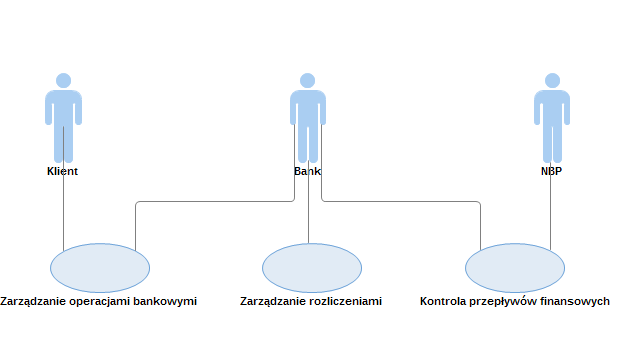
\includegraphics[width=13cm, height=10cm]{img/model_domeny_funk.png}
\caption[Model domeny funkcjonalnej dla banku FrostRes]{Model domeny funkcjonalnej dla banku FrostRes.}\label{model_domeny_funk}
\end{centering}
\end{figure}

Dotychczas w banku znajdowało się kilka podsystemów wchodzących w skład jednego większego systemu: zarządzania kontami klientów, obsługa transakcji finansowych oraz zarządzanie rozliczeniami. W przypadku banku FrostRes istotne dla wprowadzonych modyfikacji są: zarzadzanie operacjami bankowymi oraz zarządzanie rozliczeniami. Wszystkie podsystemy są zgodne z pryncypiami SOA, więc nie będzie konieczne tworzenie usług obudowujących. W późniejszym etapie metody MatSOA zostaną wykryte usługi obecnych systemów.

Do atrybutów jakościowych zalicza się przede wszystkim podstawowe zasady SOA. Stosowanie się do nich w przypadku banku FrostRes jest niebywale ważne, ponieważ w systemie planowane są częste zmiany. Musi charakteryzować się dlatego jak największą ziarnistością, reużywalnością oraz powinien być w jak największym stopniu skalowalny. 

\subsection{Wykrywanie usług}
W kolejnym etapie analizy wykonywane jest wykrywanie usług. Identyfikując usługi rozpatrujemy domeny funkcjonalne oraz zależności pomiędzy nimi kierując się utworzonym wcześniej, uproszczonym modelem procesu biznesowego. 

W pierwszym kroku wykrywania usług tworzymy wstępny model kandydatów usług jak na rys. \ref{service_candidates_init}.

\begin{figure}[h!tbp]
\begin{centering}
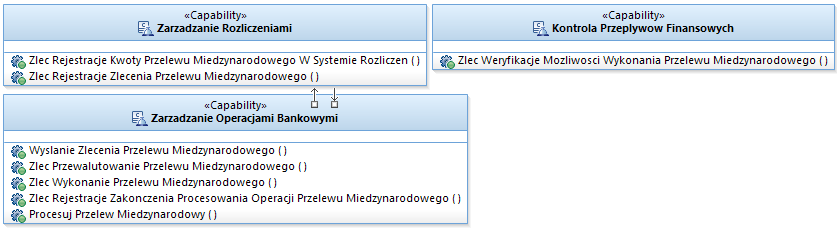
\includegraphics[width=16cm, height=5cm]{img/service_candidates_init.png}
\caption[Wykrywanie usług - wersja inicjalna]{Wykrywanie usług - wersja inicjalna}\label{service_candidates_init}
\end{centering}
\end{figure}

Na powyższym diagramie kandydatów usług można zauważyć, że do poszczególnych domen (Zarządzanie Rozliczeniami, Kontrola Przepływów Finansowych, Zarządzanie Operacjami Bankowymi) zostały przypisane odpowiednie operacje. 

Inicjalny diagram kandydatów należy rozważyć pod kątem refaktoryzacji w celu spełniania wymagań niefunkcjonalnych. Na diagramie można zauważyć, że operacja \emph{Wysłanie Zlecenia Przelewu Miedzynarodowego} jest nadmiarowa (jest wewnętrzna i nie ma wpływu na przepływ pomiędzy poszczególnymi kandydatami usług). Ponadto na diagramie nie ma metody, która odpowiadałaby za uruchomienie obsługi przelewu międzynarodowego. 

Na kolejnym diagramie (rys. \ref{service_candidates_refactored}) została dokonana refaktoryzacja inicjalnego modelu kandydatów usług. 

\begin{figure}[h!tbp]
\begin{centering}
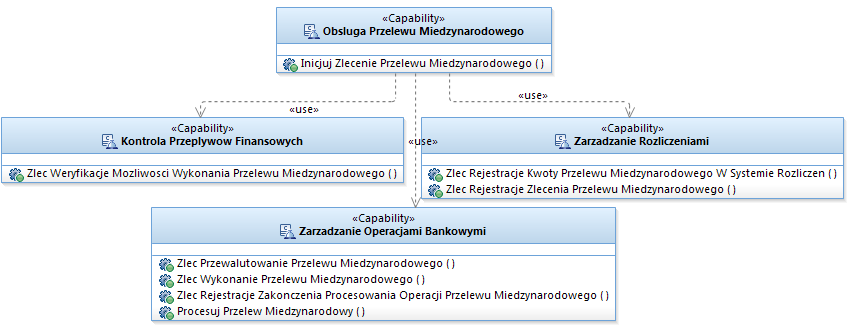
\includegraphics[width=16cm, height=7cm]{img/service_candidates_refactored.png}
\caption[Wykrywanie usług - wersja po refaktoryzacji]{Wykrywanie usług - wersja po refaktoryzacji}\label{service_candidates_refactored}
\end{centering}
\end{figure}

Została usunięta metoda nadmiarowa \emph{Wysłanie Zlecenia Przelewu Miedzynarodowego} oraz utworzony oddzielne Capability \emph{Obsluga Przelewow Miedzynarodowych} z metodą \emph{Inicjuj Zlecenie Przelewu Miedzynarodowego}.

\subsection{Wykrywanie usług obecnych systemów}
Na etapie analizy zostały wykryte dotychczasowe systemy, które występują w banku FrostRes: zarządzanie operacjami bankowymi oraz zarządzanie rozliczeniami. System banku dotychczas spełniał operacje związane z wykonywaniem przelewów krajowych oraz wpłatami i wypłatami pieniędzy z rachunka klienta. 

Na diagramie (rys. \ref{legacy_systems_service_refactored}) zostały przedstawione metody usług obecnych systemów już po wykonyanej refaktoryzacji.

\begin{figure}[h!tbp]
\begin{centering}
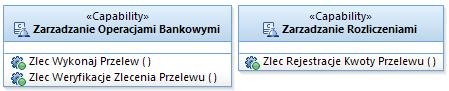
\includegraphics[width=8.5cm, height=2cm]{img/legacy_systems_services_refactored.png}
\caption[Wykrywanie usług obecnych systemów - wersja po refaktoryzacji]{Wykrywanie usług obecnych systemów - wersja po refaktoryzacji}\label{legacy_systems_service_refactored}
\end{centering}
\end{figure}

\subsection{Konsolidacja usług}
W poprzednich etapach wykryte usługi poddano konsolidacji (rys. \ref{services_consolidation}). Zauważono, że z usług systemów dotychczas występujących można uogólnić niektóre metody związane z przelewem międzynarodowym. W tym wypadku metodę \emph{Zlec Wykonanie Przelewu Miedzynarodowego} można zastąpić operację \emph{Zlec Wykonanie Przelewu}. Podobnie operację \emph{Zlec Rejestracje Kwoty Przelewu Miedzynarodowego} zastąpiono metodą \emph{Zlec Rejestracje Kwoty Przelewu}.

\begin{figure}[h!tbp]
\begin{centering}
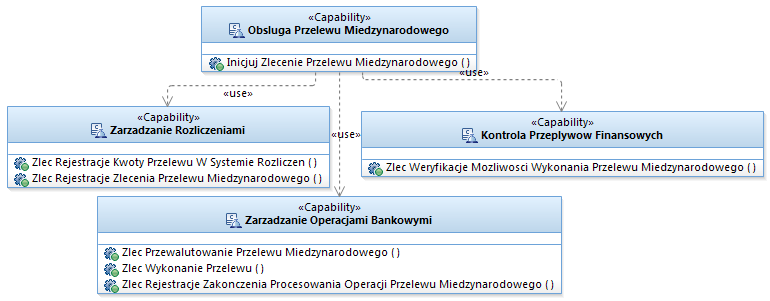
\includegraphics[width=16cm, height=7cm]{img/consolidation_services.png}
\caption[Konsolidacja usług]{Konsolidacja usług}\label{services_consolidation}
\end{centering}
\end{figure}


\subsection{Specyfikacja usług}
Przetworzone usługi w wyniku konsolidacji zgodnie z metodą MatSOA poddano w kolejnym etapie specyfikacji. W tej fazie przygotowano model danych oraz ustalono argumenty wejściowe i wyjściowe dla poszczególnych operacji interfejsów (rys. \ref{services_specification}).

\begin{figure}[h!tbp]
\begin{centering}
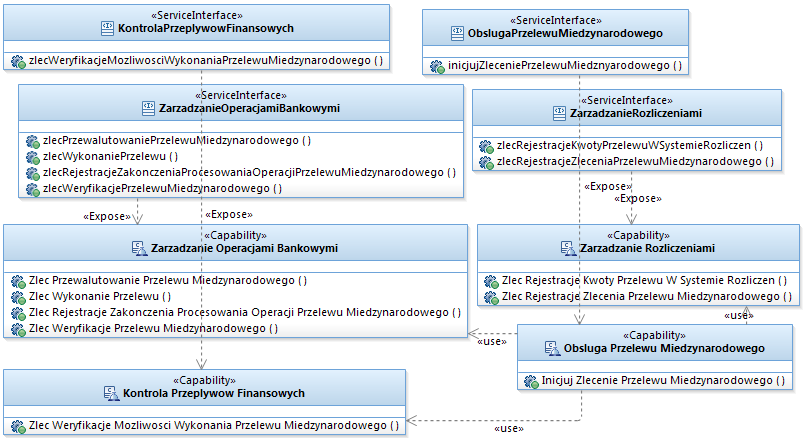
\includegraphics[width=16cm, height=9cm]{img/services_specification_model.png}
\caption[Specyfikacja usług]{Specyfikacja usług}\label{services_specification}
\end{centering}
\end{figure}

Wszystkie elementy \emph{<<Capability>>} zostały wykorzystane do utworzenia elementów \emph{<<ServiceInterface>>} przy pomocy połączenia typu \emph{<<Expose>>}. 

W przypadku specyfikacji usług dla banku FrostRes przyporządkowano do każdego elementu \emph{<<Capability>>} jeden element \emph{<<ServiceInterface>>}. Stosowanie tej praktyki nie jest zawsze konieczne. Często zdarza się możliwość przypisania więcej niż jednego elementu \emph{<<Capability>>} do jednego elementu \emph{<<ServiceInterface>>}. 

W celu bardziej szczegółowego wyspecyfikowania usług banku FrostRes przygotowano również opisy kontraktów usług oraz modele sekwencji pomiędzy poszczególnymi podmiotami w procesie. 

\subsection{Projektowanie usług}
Projektowanie usług rozpoczęto od utworzenia diagramu uczestników (ang. \emph{Participants diagram}) biorących udział w usługach. Zaznaczono na nim interfejsy dostarczane oraz wywoływane. Wyodrębniono takich uczestników jak: \emph{ZarzadcaOperacjiBankowych}, \emph{KontroloerPrzeplywowFinansowych}, \emph{ZarzadcaRozliczen}.

Na podstawie diagramu uczestników oraz specyfikacji usług przygotowano diagram komponentów dla przelewów międzynarodowych (rys. \ref{operacja_przelewu_diagram_komponentow}). Komponent posiada jeden interfejs zewnętrzny \emph{ObslugaPrzelewuMiedzynarodowego}. Poszczególne interfejsy uczestników usługi (zarówno wywoływane jak i dostarczane) zostały połączone przy użyciu elementu \emph{<<ServiceChannel>>}.

\begin{figure}[h!tbp]
\begin{centering}
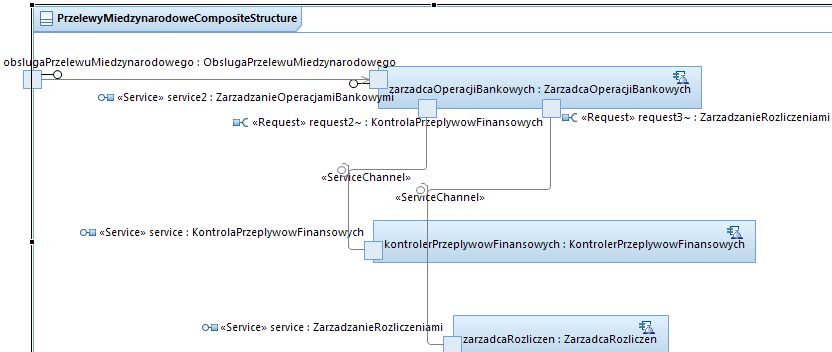
\includegraphics[width=16cm, height=8.5cm]{img/przelew_miedzynarodowy_composite.png}
\caption[Diagram komponentów dla usługi przelewu międzynarodowy]{Diagram komponentów dla usługi przelew międzynarodowy}\label{operacja_przelewu_diagram_komponentow}
\end{centering}
\end{figure}

\subsection{Choreografia usług}
Choreografia usług w formie procesu biznesowego BPEL została utworzona w narzędziu WebSphere Integration Developer. Przygotowanie procesu rozpoczęto od utworzenia diagramu asemblacji gdzie zaznaczone są usługi importowane do procesu (\emph{inbound}) oraz eksportowane (\emph{outbound}).

\section{Proces wdrożenia}
Utworzone modele usług zostały poddane transformacie UML do SOA w narzędziu Rational Software Architect. Wygenerowane zostały opisy poszczególnych usług przy wykorzystaniu WSDL oraz zdefiniowano obiekty danych za pomocą XSD (ang \emph{XML Schema Definition}). 

Wygenerowane elementy zostały następnie zaimportowane do narzędzia WebSphere Integration Developer. Utworzono w nim projekt typu \quotedblbase Rozwiązanie integracji\textquotedblright. W projekcie na diagramie asemblacji (ang. \emph{Assembly diagram}) przedstawiono komunikację pomiędzy poszczególnymi komponentami (\ref{komponenty_inbound_outbound}).  

\begin{figure}[h!tbp]
\begin{centering}
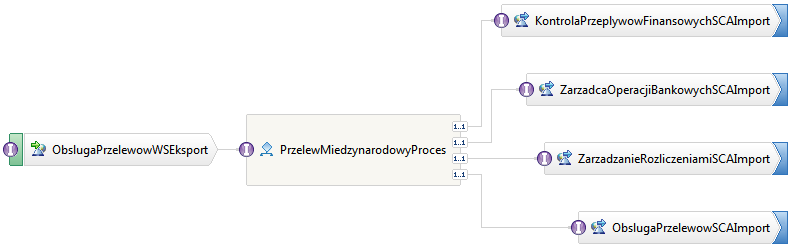
\includegraphics[width=15cm, height=5.5cm]{img/komponenty_inbound_outbound.png}
\caption[Diagram asemblacji dla przelewu międzynarodowego]{Diagram asemblacji dla przelewu międzynarodowego}\label{komponenty_inbound_outbound}
\end{centering}
\end{figure}


\section{Testy}
W celu weryfikacji poprawnego funkcjonowania, system dla banku FrostRes został poddany testom obejmujących kilka istotnych obszarów.

Testy funkcjonalne rozpoczęto od sprawdzenia poszczególnych systemów czy udzielają pożądanych odpowiedzi. Owa weryfikacja opierało się na wykonaniu bezpośrednich zapytań SOAP do każdego z systemów przy wykorzystaniu narzędzia SoapUI. Po rozważeniu otrzymanych wyników stwierdzono, że systemy zewnętrzne udzielały oczekiwanych odpowiedzi.

Po integracji z systemami wykonano test polegający na wykonaniu różnych zapytań (zmianie ulegały dane wejściowe) do usługi wystawianej przez system banku FrostRes związanej z przelewami międzynarodowymi. Stwierdzono, że wszystkie odpowiedzi są zgodne z założeniami.

Nastąpiła również próba testów z poziomu interfejsu strony. Wypełniano formularz i sprawdzano czy interakcja ze strony systemu będzie poprawna (rys. \ref{test_funk_interfejs}). 

\begin{figure}[h!tbp]
\begin{centering}
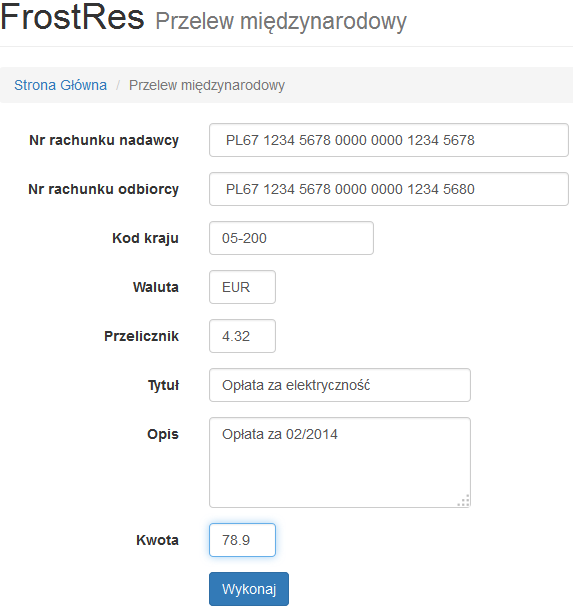
\includegraphics[width=8cm, height=9.5cm]{img/przelew_wypelniony_form.png}
\caption[Testy z poziomu interfejsu - formularz przelewu międzynarodowego]{Testy z poziomu interfejsu - formularz przelewu międzynarodowego}\label{test_funk_interfejs}
\end{centering}
\end{figure}


Testy niefunkcjonalne, którym został poddany system obejmowały głównie obszar związany z wydajnością systemu. Do przeprowadzenia testów wydajnościowych zastosowano narzędzie LoadUI. 

Wyniki przeprowadzonych testów umieszczono w tab. \ref{tabela_stat_wyd}. Poszczególne czasy odpowiedzi na zapytania związane ze zleceniem przelewu międzynarodowego okazały się bardzo krótkie (średni czas odpowiedzi wyniósł 424,22). Ponadto w ciągu 10 sekund bank jest w stanie obsłużyć aż blisko 63 przelewy międzynarodowe. Stanowi to o wysokim poziomie wydajności systemu. Należy wziąć jednak pod uwagę, że uruchomiony system integrował się z aplikacjami zaślepiającymi docelowe systemy. W przypadku integracji z prawdziwymi systemami różnice w czasach odpowiedzi mogłyby wynikać z faktu obsługi komponentów przez różne architektury fizyczne oraz opóźnień w połączeniach sieciowych.

\begin{table}[!htbp]
\begin{center}
\begin{small}
\begin{supertabular}{|p{3cm}|p{3cm}|p{3cm}|p{4cm}|}\hline
\textbf{Min. czas odp. [ms]} & \textbf{Max czas odp. [ms]} & \textbf{Śr. czas odp. [ms]} & \textbf{Ilość odp. w ciągu 10 s.}\\\hline
215 &	998 & 424,22 & 63  \\\hline
\end{supertabular}
\end{small}
\end{center}
 \caption{Statystyki wydajnościowe systemu dla banku FrostRes.}
 \label{tabela_stat_wyd}
\end{table}


\section{Cel systemu w odniesieniu do zaprojektowanej koncepcji}
Zaprojektowana koncepcja umożliwiła utworzenie systemu zgodnego z paradygmatami SOA przy wykorzystaniu języka SoaML. Przykładowy system posiadał niezbyt skomplikowane wymagania funkcjonalne jednakże metodę MatSOA równie dobrze można by przełożyć na bardziej złożone systemy.

Cel systemu został w pełni osiągnięty. Przede wszystkim charakteryzuje się bardzo wysokim stopniem skalowalności, ponieważ można go łatwo rozbudowywać poprzez dołączanie nowych komponentów. Ponadto pomiędzy poszczególnymi elementami systemu występują luźne powiązania. Każdy z komponentów może działać niezależnie od pozostałych.

Inne zasady SOA takie jak reużywalność, interoperacyjność czy kontraktowość również zostały spełnione. Każdy komponent systemu może być wykorzystany w kontekście innego systemu. Zasada interoperacyjności została uwzględniona, ponieważ system banku FrostRes może z powodzeniem komunikować się z pozostałymi systemami (jak na przykład opisywany NBP). Ponadto pomiędzy usługami, a konsumentami widać wyraźnie zdefiniowane kontrakty (kontraktowość usług).

\chapter{Podsumowanie i wnioski}
\TODO: Wyciągnięcie wniosków wraz z podsumowaniem

\begin{thebibliography}{99}
\addcontentsline{toc}{chapter}{Bibliografia}
\bibitem{SOMAArsIBMJour}{Arsanjani Ali, \emph{IBM Systems Journal}, wyd. 47, nr 3, 2008.}
\bibitem{ArchWhatIs}{Autor nieznany, \url{http://www.archimate.nl/en/about_archimate/what_is_archimate.html}.}
\bibitem{EfektyZasSys}{Autor nieznany , \url{http://mfiles.pl/pl/index.php/Efekty_wdra\%C5\%BCania_informatycznych_system\%C3\%B3w_zarz\%C4\%85dzania.}}
\bibitem{SOAManifestoOrg}{Autor nieznany , \url{http://www.soa-manifesto.org/.}}
\bibitem{SOAawidptas}{Bean J., \emph{and Web Services Interface Design: Principles, Techniques, and Standard}, Morgan Kaufmann Publishers, 2010.}
\bibitem{EntSOACoryCanSoaML}{Casanave Cory, \emph{Enterprise Service Oriented Architecture - using the OMG SoaML Standard}, Model Driven Solutions, 2009.}
\bibitem{SOAwJBBC}{Binildas A. Christudas, Malhar Balai, Caselli Vincenzo, \emph{Service Oriented Architecture with Java: Using SOA and Web Services to Build Powerful Java Applications}, Packt Publishing, 2008.}
\bibitem{SoaMLErvBase}{\emph{Specyfing services using the Service Oriented Architecture modeling language (SoaML): A baseline for specification of Cloud-based Services}, Elvesæter Brian, Berre Arne-Jørgen, Sadovykh Andrey, In CLOSER, 2011}
\bibitem{IBMRBSoaPat}{Endrei Mark, Ang Jenny, Arsanjani Ali, Sook Chua, Comte Philippe, Krogdahl Pål, Luo Min, Newling Tony, \emph{Patterns: Service-Oriented Architecture and Web Services}, IBM, 04/2004.}
\bibitem{RUPMartFow}{Fowler Martin, \url{http://www.martinfowler.com/articles/newMethodology.html.}}
\bibitem{PlatIntGor}{Górski Tomasz, \emph{Platformy integracyjne. Zagadnienia wybrane}, Wydawnictwo naukowe PWN, 2012.}
\bibitem{TopDownArchimate}{Graves Tom, \url{http://weblog.tetradian.com/2011/07/26/from-biz-model-to-ea/}.}
\bibitem{JonSimRUPSoa}{Johnson Simon, \emph{Tooling platforms and RESTful ramblings} \url{https://www.ibm.com/developerworks/community/blogs/johnston/entry/rup_for_soa_and_soma?lang=en}, 2006.}
\bibitem{JosSOAHist}{Josuttis Nicolai, \emph{SOA in Practice: The Art of Distributed System Design}, O'Reillyl, 2007}
\bibitem{RUPIntRat}{Kruchten Philippe, \emph{The Rational Unified Process: An Introduction}, Addison-Wesley Professional, 12/2003.}
\bibitem{SOAMLOMG}{OMG contributors, \emph{Service oriented architecture Modeling Language (SoaML) Specification},OMG, 03/2012.}
\bibitem{OffCompSOAM}{Offermann Philipp, Udo Bub, \emph{Empirical comparison of methods for information systems development according to SOA}, Deutsche Telekom Laboratories, 2009.}
\bibitem{PapaZog}{Papazoglou Michael, \emph{Service-Oriented Design and Development Methodology}, INFOLAB, 2005.}
\bibitem{ArchKorpAdmPub}{Proppe Mirosław, Suchorzewska Aleksandra, \emph{Architektura korporacyjna w administracji publicznej}, \url{https://www.kpmg.com/PL/pl/IssuesAndInsights/ArticlesPublications/Documents/Architektura\%20Korporacyjna\%20w\%20administracji\%20publicznej_secured.pdf.}}
\bibitem{RamErvSOA}{Ramollari Ervin , A Survey of Service Oriented Development Methodologies, 2007}
\bibitem{SOAWzorceArch}{Rotem-Gal-Oz Arnon, \emph{Wzorce SOA}, Helion, 2013.}
\bibitem{ArchKorpSob}{Sobczak Andrzej, \emph{Architektura korporacyjna. Aspekty praktyczne i wybrane zagadnienia teoretyczne}, Ośrodek Studiów nad Cyfrowym Państwem, 2013.}
\bibitem{SobArchKorpDobrPr}{Sobczak Andrzej, \emph{Kodeks dobrych praktyk architektów korporacyjnych}, \url{http://architekturakorporacyjna.pl/kodeks-dobrych-praktyk-architektow-korporacyjnych/1683/.}}
\bibitem{SobArchKorpProg}{Sobczak Andrzej, \emph{Kodeks dobrych praktyk architektów korporacyjnych}, \url{http://architekturakorporacyjna.pl/architektura-korporacyjna-w-roku-2015-prognoza/5508/.}}
\bibitem{SteveMichSOA}{Stevens Michael, \emph{Service Oriented Architecture Introduction}, \url{http://architekturakorporacyjna.pl/kodeks-dobrych-praktyk-architektow-korporacyjnych/1683/}, 2012}
\bibitem{SOMAibmRosSuda}{Suda Michał, Marcin Roszczyk, \emph{Projektowanie Modeli Usług dla rozwiązańtypu SOA}, IBM, 2006.}
\bibitem{CompSOAMet}{Svanidaite Sandra, \emph{A Comparison of SOA Methodologies Analysis \& Design Phases}, Institute of Mathematics and Informatics, 2012.}
\bibitem{SOAsdj102009}{Wasiukiewicz Radosław, \emph{SOA, czyli Service Oriented Architecture}, Software Developer Journal, 10/2009.}
\bibitem{ArchKorpSzymSup}{Supernak Szymon, \emph{Wprowadzenie do modelowania architektur korporacyjnych w usługach publicznych}. Zeszyty Naukowe Nr 4, WWSI, 2010.}
\bibitem{OpenGrArch}{The Open Group, \url{http://www.opengroup.org/subjectareas/enterprise/archimate}.}
\bibitem{BMMOmg}{OMG, \emph{Business Motivation Model - specification}, 05/2010}
\bibitem{AnaWesHal}{Wesołowska Halina, \url{http://analizait.pl/2013/business-motivation-model-po-coz-my-to-robimy}, 05/2013.}
\bibitem{MicMetZIMM}{Zimmermann Olaf, Koehler Jan, Leymann Frank, \emph{Architectural Decision Models as Micro-Methodology for Service-Oriented Analysis and Design}, Zurich Research Laboratory, 2007}
\end{thebibliography}
\end{document}
